\documentclass[letterpaper]{article} % DO NOT CHANGE THIS
% AAAI-27 Author Kit (official, https://aaai.org/authorkit27/, AuthorKit27.zip, aaai2027.sty dated 2026-10-21).
% Anonymous-submission mode; author information is a placeholder pending the user's decision.
\usepackage[submission]{aaai2027}  % DO NOT CHANGE THIS
\usepackage[hyphens]{url}  % DO NOT CHANGE THIS
\usepackage{graphicx} % DO NOT CHANGE THIS
\urlstyle{rm} % DO NOT CHANGE THIS
\def\UrlFont{\rm}  % DO NOT CHANGE THIS
\usepackage{natbib}  % DO NOT CHANGE THIS AND DO NOT ADD ANY OPTIONS TO IT
\usepackage{caption} % DO NOT CHANGE THIS AND DO NOT ADD ANY OPTIONS TO IT
\frenchspacing  % DO NOT CHANGE THIS
\usepackage{algorithm}
\usepackage{algorithmic}
\usepackage{booktabs}
\usepackage{array}
\usepackage{amsmath}
\usepackage{placeins} % \FloatBarrier keeps appendix floats in their sections
\pdfinfo{
/TemplateVersion (2027.1)
}
\setcounter{secnumdepth}{2} % Section numbers enabled (permitted by the template: 0, 1 or 2).

\title{BrickForma: Text-to-Brick Generation with Voxel-to-Brick Data Construction and Geometric Reconstruction}
\author{
    % TODO 待用户确认: author names and affiliations are placeholders until the user provides them.
    Author Name(s) to Be Added\textsuperscript{\rm 1}
}
\affiliations{
    \textsuperscript{\rm 1}Affiliation(s) to Be Added\\
    email@to-be-added
}

\begin{document}

\maketitle

\begin{abstract}
Generating brick structures from text requires geometric assembly: bricks must fit in a bounded grid, avoid overlaps, and interlock through studs, not merely resemble the described shape. We study how far a language model can learn such a spatial representation from programmatically generated data. Using GPT-6.1 Sol, an agentic batch-generation pipeline writes parametric generator programs that emit 80,000 voxel models across 21 categories on a $48^3$ grid, each with five bilingual captions of increasing detail. Same-color tiling, connectivity analysis, and local bridging and retiling convert the shapes into brick layouts, and 79,301 models pass the specified geometric checks. We fine-tune Qwen3-1.7B with LoRA on English captions and serialized brick placements, and repair its predictions by solving a shape-preserving exact cover with a single stud-connected component via mixed-integer linear programming (MILP). A structural analysis of raw outputs shows that interlocking across layers is the constraint the learned representation most often misses. On 114 shared prompts under a common rendering protocol, the evaluated BrickForma outputs (110 retiled, 4 raw) obtain the highest mean scores on three text--image alignment metrics and a mean invalid-placement ratio of 0.00\%, matching BrickGPT.
\end{abstract}

\begin{figure*}[t]
\centering
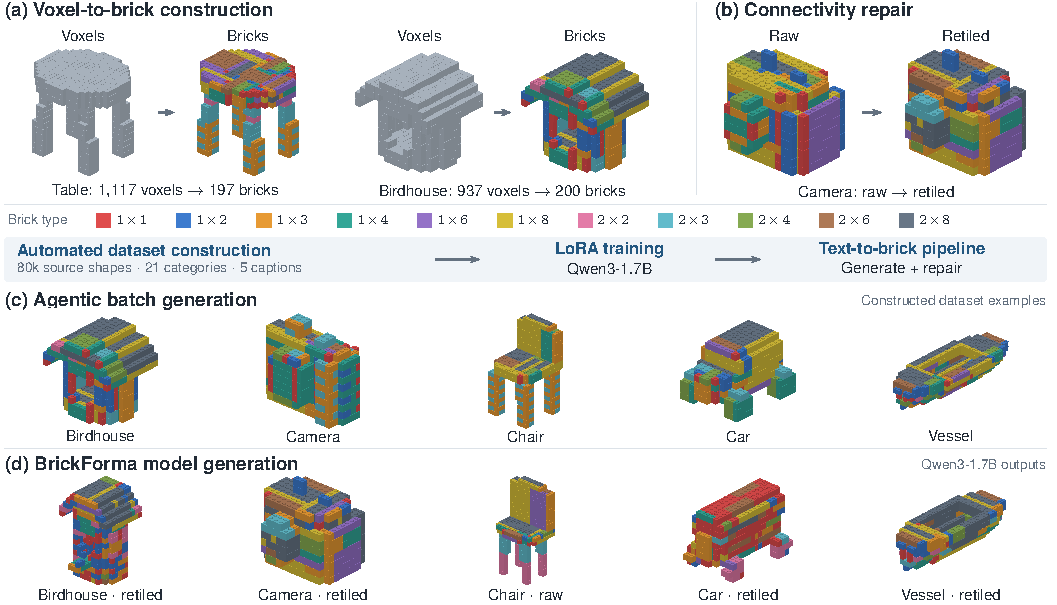
\includegraphics[width=0.94\textwidth]{figure1.pdf}
\caption{\textbf{BrickForma overview.} (a) Source voxels are converted into rectangular bricks. (b) Raw predictions are retiled to repair connectivity. (c) Constructed brick layouts from agentically generated voxel data. (d) Outputs of the fine-tuned Qwen3-1.7B pipeline. Colors encode brick type independent of orientation; they are visualization labels, not predicted appearance. Voxels are shown in gray.}
\label{fig:teaser}
\end{figure*}

\section{Introduction}
Text-to-3D generation lets users describe and create objects in natural language~\cite{dreamfusion}. Generating brick structures adds the requirement that a target shape be represented as discrete pieces and their spatial placements. Beyond matching the text, the structure must avoid overlaps and keep the bricks connected: a layout may resemble the described object while containing intersecting bricks or disconnected parts. The setting is therefore one of geometric reasoning and object assembly, in which the system must decide how bricks fit, interlock, and remain connected in space, not only whether the overall shape resembles the described object. This makes text-to-brick generation a useful testbed for learning spatial representations: the target is discrete, the constraints are exactly checkable, and a model's errors can be measured geometrically rather than only perceptually.

Prior work has explored text-driven brick generation with different representations and constraints. BrickGPT trains an autoregressive language model on paired text and brick structures and applies validity checks and physics-aware rollback during inference~\cite{brickgpt}. BrickNet uses a graph-backed representation to generate assembly sequences over a broader range of parts and connection types~\cite{bricknet}. Both show that structural representations and generation-time constraints matter for brick modeling.

For voxel-based shapes, spatial adjacency between voxels does not imply a valid connection between bricks: a voxel shape can form one connected volume even when the bricks covering it only touch side by side without stud connections. This distinction affects both data construction and generation. Converting voxel shapes into training targets requires attention to coverage and stud connectivity, and predicted layouts may contain overlaps or disconnected components that require further processing.

We present BrickForma to study this problem. GPT-6.1 Sol writes parametric generator programs that emit voxel models in batches; a conversion pipeline tiles them with same-color bricks and uses local bridging and retiling to address ungrounded components, recording any change to the source voxels. We then fine-tune Qwen3-1.7B~\cite{qwen3} with LoRA~\cite{lora} on English captions and brick-placement sequences, so that the $48^3$ workspace, multi-level captions, and fixed spatial serialization define the representation being learned. Because the model's raw layouts may still overlap or fall apart into stud-disconnected pieces, a post-generation stage forms the voxel union of supported placements, seeks an exact cover with a single stud-connected component by MILP, and queues a new sampling seed when no cover is found within the solver budget. The connectivity check is geometric; physical stability and assembly-order feasibility require separate evaluation.

Our analysis asks what such a model actually learns from generated data. A diagnostic analysis of raw outputs (Section~\ref{sec:diagnostics}) shows that the model's layouts usually fail to interlock across layers and fall apart into several stud-connected pieces. We therefore treat geometric repair as a complement to, not a substitute for, the learned representation, and we report both raw and retiled results.

We compare the provided outputs of BrickForma, BrickGPT, and BrickNet on 114 shared prompts spanning 21 categories and five description levels, measuring text--image alignment with VQAScore, PE, and SigLIP2 and the invalid-placement ratio $P_{\mathrm{inv}}$. Under a common rendering protocol, BrickForma has the highest mean on all three alignment metrics, and BrickForma and BrickGPT both have a mean $P_{\mathrm{inv}}$ of 0.00\% in exported file order. The ordering holds at every description level from L1 to L5 (Appendix~\ref{app:eval}). These results describe the provided outputs under the stated protocol and do not by themselves establish physical stability or assembly feasibility.

Our contributions are as follows.
\begin{enumerate}
\item \textbf{Data generation for spatial learning.} An agentic batch-generation pipeline in which GPT-6.1 Sol writes parametric generator programs, producing 80,000 $48^3$ voxel models across 21 categories with five bilingual captions each, and a voxel-to-brick conversion that targets stud-connected layouts rather than voxel adjacency; 79,301 models pass the specified geometric checks.
\item \textbf{Fine-tuned text-to-brick representation.} LoRA fine-tuning of Qwen3-1.7B on serialized placements over a 20-type library in a $48^3$ workspace, with post-generation MILP retiling that enforces a single stud-connected component.
\item \textbf{Geometric diagnosis and evaluation.} A structural analysis of raw outputs on 525 prompts showing which spatial constraints the model learns and which it misses, and a matched comparison with BrickGPT and BrickNet on 114 prompts under a common rendering protocol.
\end{enumerate}


\begin{figure*}[t]
\centering
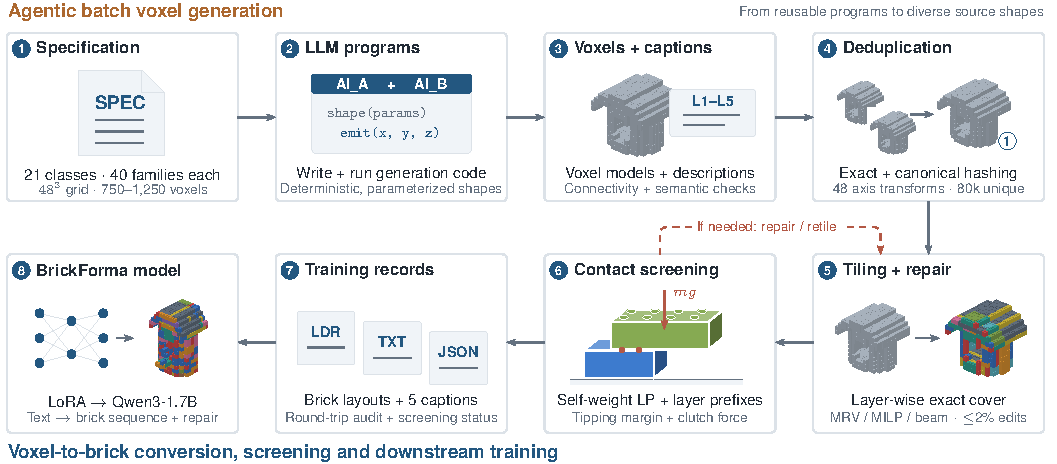
\includegraphics[width=0.94\textwidth]{figure2.pdf}
\caption{\textbf{Data-construction workflow.} GPT-6.1 Sol writes parametric programs that produce voxel shapes and captions. Deduplication, same-color tiling, local repair, and geometric checks yield layouts for fine-tuning. Contact screening is recorded separately. The dashed arrow denotes further repair or retiling. Brick colors follow the legend in Figure~\ref{fig:teaser}.}
\label{fig:data-workflow}
\end{figure*}

\section{Related Work}
\paragraph{Brick assembly and generation.}
Learning-based brick construction has been studied as graph generation~\cite{thompson2020lego}, as combinatorial construction with deep reinforcement learning~\cite{brickbybrick}, and as interactive structural understanding in a LEGO simulator~\cite{breakandmake}. For text-conditioned generation, BrickGPT represents a design as an autoregressively generated sequence of brick placements and uses brick-level rejection sampling with physics-aware rollback at inference~\cite{brickgpt}; BrickNet represents part connectivity through a graph-backed parametrization and trains autoregressive models on its assembly sequences~\cite{bricknet}. BrickForma also generates placement sequences from text, on a larger $48^3$ grid with a 20-type library, and examines geometric reconstruction and connectivity in a separate post-generation stage.

\paragraph{Stability analysis.}
StableLego analyzes the structural stability of block-stacking assemblies with a force-balance optimization~\cite{stablelego}. Such analyses depend on their mechanical assumptions. In BrickForma, geometric connectivity and the contact-based screening in the dataset materials address different properties; neither alone establishes that every generated model can be physically assembled and remains stable.

\paragraph{Procedural data and parameter-efficient fine-tuning.}
Procedural generation is a common way to obtain large, controllable 3D training data~\cite{infinigen}. BrickForma uses a language model to write the procedural generators rather than to emit coordinates directly. The text-to-brick model is adapted with LoRA~\cite{lora}, following the BrickGPT recipe of fine-tuning a pretrained language model on serialized brick sequences~\cite{brickgpt}.

\paragraph{Language models for serialized 3D structure.}
Autoregressive transformers can generate 3D geometry as token sequences, e.g., triangle meshes in MeshGPT~\cite{meshgpt}; LLaMA-Mesh fine-tunes a pretrained language model to emit meshes as plain text~\cite{llamamesh}. BrickGPT and BrickForma apply the same idea to discrete brick placements, where validity can be checked exactly.

Synthetic spatial data is also used to teach vision--language models spatial relations, e.g., SpatialVLM~\cite{spatialvlm}; BrickForma instead trains a text-only generator on programmatically generated assembly data and uses vision--language models only for evaluation.

\section{Dataset Construction}
\label{sec:dataset}
\subsection{Parametric Voxel Generation}
BrickMore-48 contains 80,000 voxel models on a $48^3$ grid across 21 categories (3,805--3,810 per category), each paired with five bilingual captions at levels L1 (concise) to L5 (detailed); for example, the L1 caption of one birdhouse model reads ``An oval birdhouse with curved roof, enclosed room and front entrance.'', and its L5 caption extends this with structure, proportions, color regions, and views (Appendix~\ref{app:dataset}). The models are produced by parametric generator programs written through agentic batch generation with GPT-6.1 Sol; the programs, rather than the language model itself, emit the voxel coordinates. Each record includes a geometry plan and a dataset version identifier for reproduction, and exact and canonical (48 axis/sign transforms) occupancy hashes show no duplicates across the two 40,000-model shards. Figure~\ref{fig:data-workflow} summarizes the workflow; sample shapes are shown in Appendix~\ref{app:dataset}.


\subsection{Voxel-to-Brick Conversion and Checks}
The conversion pipeline tiles occupied voxels with same-color rectangular bricks and analyzes their connections. Relative to the earlier relaxed release, the local bridging-and-retiling stage raises the number of geometrically passing models from 65,503 to 79,298 (13,795 recovered failures) while adding 228,582 and removing 125 voxels in total across the corpus; 31,532 passing models require no voxel change at all. Local bridging and retiling address ungrounded components, and changes to source voxels are recorded separately. Each converted model carries a \texttt{validation.json} that records three geometric constraints: the occupied voxels form a single six-neighbor connected component, every brick component is grounded, and the bricks exactly cover the (derived) target voxels. Under these release rules a layout may consist of several brick components that are each grounded; this criterion differs from the single stud-connected component enforced by post-generation retiling (Section~\ref{sec:model}). The dataset materials also describe a contact-based gravity screening procedure; its outputs are screening results under stated assumptions rather than proof of physical stability (Appendix~\ref{app:dataset}); training-data selection uses the geometric checks.

\subsection{Integrated Release and Training Corpus}
The full retile release records 79,298 geometrically passing models; the 702 failures (0.88\%) are concentrated in table (132), bookshelf (110), vessel (89), bowl (79), and bus (75). Replacing all 1,905 batch-B piano slots (1,902 passing) with a regenerated release in which all 1,905 pass gives an integrated count of $79{,}298-1{,}902+1{,}905=79{,}301$ passing models. This number is computed from the two release reports, not from a new full-dataset verification run, and the original A/B download does not apply the replacement automatically. Fine-tuning uses only geometrically passing models (Table~\ref{tab:training-data}).

\begin{table}[t]
\centering
\small
\setlength{\tabcolsep}{4pt}
\begin{tabular}{lr}
\toprule
\multicolumn{2}{l}{\emph{Dataset (release reports)}} \\
\midrule
Source models / categories / grid & 80,000 / 21 / $48^3$ \\
Bilingual caption records & 400,000 \\
Failing in full retile release & 702 (0.88\%) \\
Passing in full retile release & 79,298 \\
Piano models restored by revised release & 3 \\
Integrated passing models & 79,301 \\
\midrule
\multicolumn{2}{l}{\emph{Fine-tuning corpus}} \\
\midrule
(model, English caption) samples & 396,610 \\ % 待用户确认 (U3)
Training / validation samples & 356,955 / 39,655 \\
Tokens over 3 epochs & 2,228,044,818 \\ % 待用户确认 (U3)
\bottomrule
\end{tabular}
\caption{Dataset and fine-tuning corpus. The two blocks are counted separately: the upper block from the dataset release reports, the lower block as recorded for the fine-tuning run.}
\label{tab:training-data}
\end{table}

\section{BrickForma Text-to-Brick Model}
\label{sec:model}
\subsection{Fine-Tuning}
\label{sec:training}
We fine-tune Qwen3-1.7B on BrickMore-48 with a library of 20 brick types. Relative to StableText2Brick used by BrickGPT ($20^3$, 14 types), the library adds six footprints ($3{\times}2$, $2{\times}3$, $3{\times}1$, $1{\times}3$, $2{\times}8$, $8{\times}2$). Each object occupies 750--1,250 voxels with coordinates in $\{0,\ldots,47\}$. Training uses only the English captions (\texttt{captionEn}, L1--L5); the Chinese captions are not used. Samples are split by model at a 9:1 ratio, so the captions of one model never straddle the split. Together, the fixed $48^3$ coordinate frame, the 20-type library, and a line-per-brick serialization define the representation the model learns: each line commits to one footprint and one absolute position, so library membership, bounds, and overlaps can be checked exactly line by line. The current output does not include color.

Each sample is a three-turn chat, structurally identical to the official BrickGPT data-preparation script: a system prompt (``You are a helpful assistant.''), a user instruction adapted to the $48^3$ world that lists the 20 allowed dimensions, and an assistant reply with one brick per line, e.g.\ $2{\times}4\ (x,y,z)$. No thinking content is used; inference sets \texttt{enable\_thinking=False} to match training. Brick dimensions are serialized Y-first, then X, which differs from the StableText2Brick convention; training and inference share this convention, and downstream parsers must restore the orientation consistently.

Hyperparameters follow the Qwen3 fine-tuning script in the official BrickGPT repository (Table~\ref{tab:finetune-config}) rather than the LLaMA numbers in the original paper; Appendix~\ref{app:training} compares the two. Sequences are unpacked so that each caption--sequence boundary is preserved, and dependencies are pinned to the official TRL~0.17 stack. Training runs 133,860 steps in 25.3 hours ($\approx$202 GPU-hours). Validation loss, computed every 500 steps on a 2,000-sample validation subset, reaches its minimum of 0.0308 at step 79,000 (epoch 1.77) and rises to 0.0339 by the end of epoch 3. Because \texttt{load\_best\_model\_at\_end} is enabled, the released weights are those of step 79,000, so the additional third epoch does not degrade the released model. Selected validation-loss checkpoints are listed in Appendix~\ref{app:training}.

\begin{table}[t]
\centering
\small
\setlength{\tabcolsep}{3pt}
\begin{tabular}{@{}l>{\raggedright\arraybackslash}p{0.58\linewidth}@{}}
\toprule
Item & Value \\
\midrule
Base model & Qwen3-1.7B (bf16) \\
Adaptation & LoRA, $r=16$, $\alpha=32$, dropout $0.05$, all linear layers \\
Optimization & LR $10^{-4}$, cosine, 100 warm-up steps, 3 epochs \\
Batch / max length & effective 8 (8 GPUs $\times$ 1) / 8,192 \\
Hardware & DDP, 8$\times$RTX 4090D (24\,GB) \\
Released checkpoint & step 79,000 (best validation loss) \\
Software & transformers 4.51.3, trl 0.17.0, peft 0.15.2 \\
\bottomrule
\end{tabular}
\caption{Fine-tuning configuration (details in Appendix~\ref{app:training}).}
\label{tab:finetune-config}
\end{table}

\begin{figure*}[t]
\centering
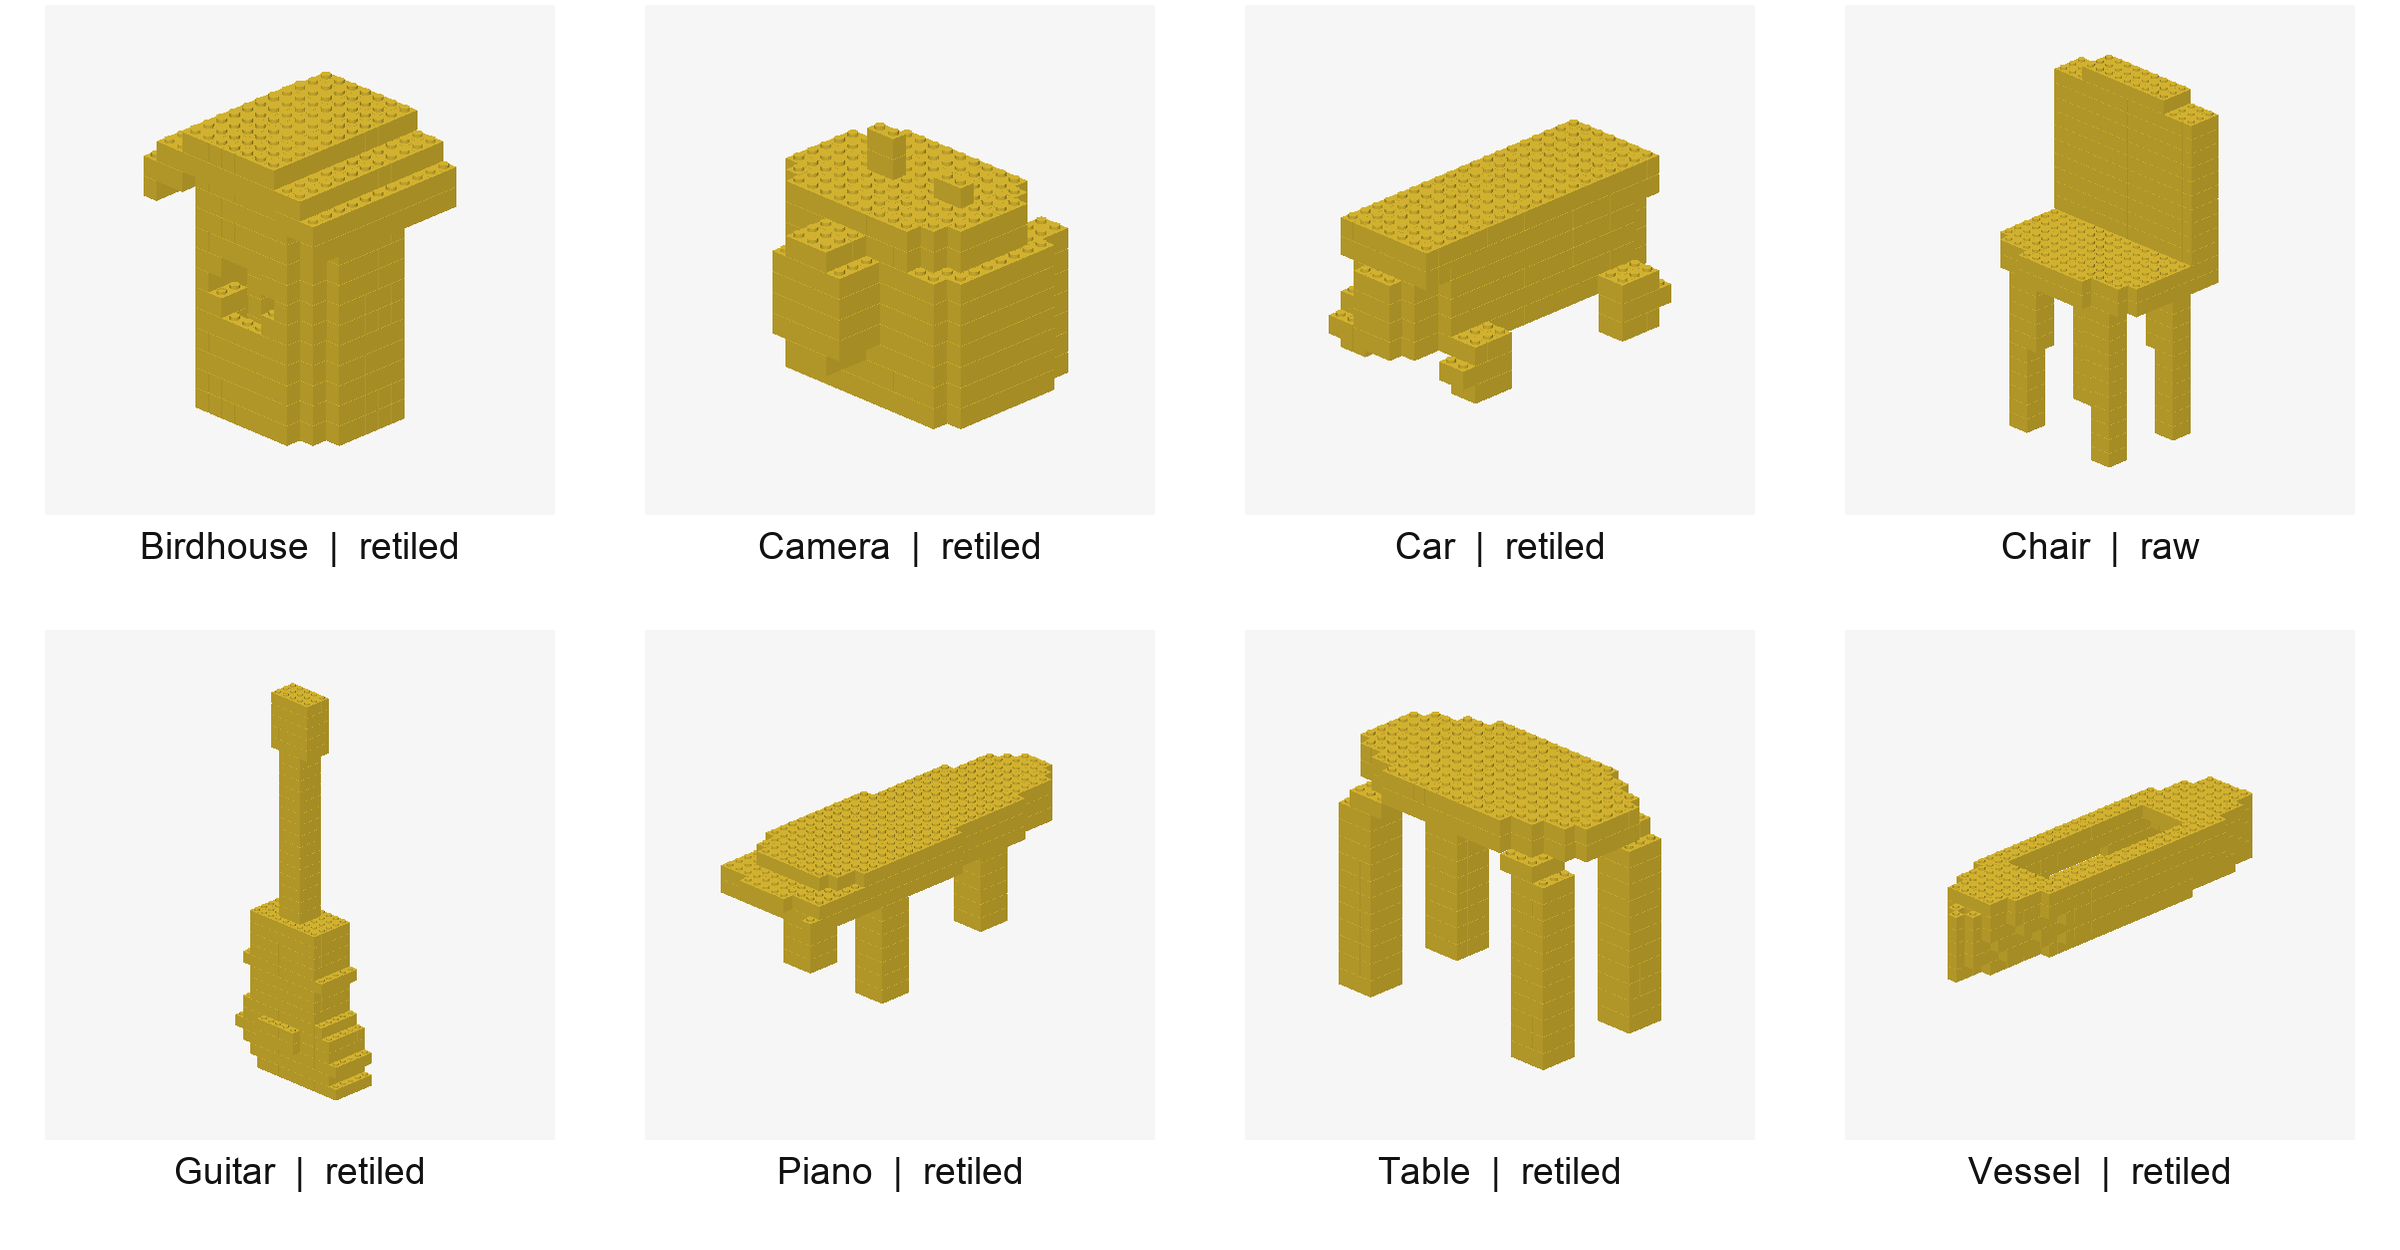
\includegraphics[width=0.75\textwidth]{figures/generated_gallery.png}
\caption{Selected BrickForma outputs from the 114-prompt evaluation, rendered with the uniform evaluation protocol (not photographs of physical assemblies). In this gallery, one chair is raw and the other outputs are retiled; in the full main comparison, 4 of the 114 BrickForma outputs are raw.}
\label{fig:gallery}
\end{figure*}

\subsection{Inference and Retiling}
Inference follows the seed-escalation and repair procedure in Algorithm~\ref{alg:inference-retiling}. The model samples a placement sequence with thinking disabled, temperature $0.7$, top-$p$ $0.9$, and at most $8192$ new tokens, using seeds $42$, $104$, and $2026$ in order. A candidate is accepted when generation completes (ends with an end-of-sequence token) and the geometry validator reports no errors. Otherwise, the pipeline keeps the completed draft with the fewest validator error records $\mathrm{Err}(\cdot)$ (line format, library membership, bounds, and overlaps). It then forms the voxel union $C$ of the in-bounds cells of supported library placements, solves a shape-preserving exact cover of $C$ with a single stud-connected component by MILP under a $12$--$60$--$180$\,s time ladder, and audits the result independently. If no cover is found within this budget, the raw draft is retained and a new seed may be queued. A separate recovery path may extend the budget to $600$\,s and sample seeds outside $S$; it is not part of the default loop. We call the MILP output the \emph{retiled} layout (files are named \texttt{stitched}) and the model's draft the \emph{raw} layout. Section~\ref{sec:diagnostics} reports how often each repair tier is reached.

\begin{algorithm}[t]
\caption{BrickForma inference and retiling}
\label{alg:inference-retiling}
\small
\begin{algorithmic}[1]
\REQUIRE prompt $c$; fine-tuned model $\theta$; library $\mathcal{L}$ (20 types); seeds $S=(42,104,2026)$; MILP tiers $T=(12,60,180)$\,s
\ENSURE $(B_{\mathrm{out}}, \textit{status})$, $\textit{status}\in\{\textsc{Success},\textsc{Draft},\textsc{Failed}\}$
\STATE $B \gets \emptyset$; $A \gets \emptyset$
\FOR{$s \in S$}
  \STATE $(B_s,\textit{rep}) \gets \mathrm{Parse}(\theta.\mathrm{Generate}(c,\ \mathrm{seed}{=}s))$
  \STATE $A \gets A \cup \{(B_s,\textit{rep})\}$
  \IF{$\textit{rep}.\mathrm{complete} \land \textit{rep}.\mathrm{valid}$}
    \STATE $B \gets B_s$; \textbf{break}
  \ENDIF
\ENDFOR
\IF{$B=\emptyset$}
  \IF{no completed draft in $A$}
    \RETURN $(\emptyset,\ \textsc{Failed})$
  \ENDIF
  \STATE $B \gets \arg\min_{\text{completed } a\in A} \mathrm{Err}(a)$
\ENDIF
\IF{$\mathrm{Err}(B)=0 \land \mathrm{StudComponents}(B)=1$}
  \RETURN $(B,\ \textsc{Success})$ \COMMENT{keep a valid connected raw layout}
\ENDIF
\STATE $C \gets \mathrm{UnionVoxels}(B;\ \mathcal{L},\ 48^3)$ \COMMENT{clip; overlaps count once}
\FOR{$\tau \in T$}
  \STATE $B^{*} \gets \mathrm{MILP\text{-}SingleStudCover}(C,\ \tau)$
  \IF{$B^{*}\neq\emptyset \land \mathrm{Audit}(B^{*},C)$}
    \RETURN $(B^{*},\ \textsc{Success})$
  \ENDIF
\ENDFOR
\STATE $\mathrm{QueueReseed}(c)$
\RETURN $(B,\ \textsc{Draft})$ \COMMENT{unsolved: keep raw draft}
\end{algorithmic}
\end{algorithm}

\section{Comparative Evaluation}
\label{sec:eval}
\subsection{Setup and Metrics}
\label{sec:setup}
We compare the provided outputs of BrickForma, BrickGPT, and BrickNet on 114 shared prompts covering 21 categories and five description levels (one output per system and prompt). For BrickForma, the provided output uses the retiled layout when available: 110 of the 114 outputs are retiled and 4 are raw. All systems are rendered with the same protocol: uniform yellow material, $512{\times}512$ orthographic views at $25^{\circ}$ elevation and eight azimuths ($0^{\circ}$ to $315^{\circ}$ in $45^{\circ}$ steps).

\emph{Text--image alignment.} VQAScore~\cite{vqascore} is the full-vocabulary softmax probability that Qwen2.5-VL-7B-Instruct~\cite{qwen25vl} generates the single token ``Yes'' as its first answer token when asked whether a rendered view shows the prompt. PE is the cosine similarity between L2-normalized image and text embeddings of PE-Core-bigG-14-448~\cite{pe}, and SigLIP2 is the sigmoid of the image--text logit of SigLIP2 giant-opt-patch16-384~\cite{siglip2}; their text encoders read at most 72 and 64 tokens, respectively. For each metric, a model's score is the maximum over its eight views, averaged over prompts. The three metrics therefore live on different scales and are compared only within a metric.

\emph{Invalid placements.} For a model with placements $b_1,\ldots,b_n$ in exported file order,
\begin{equation}
P_{\mathrm{inv}} = \frac{1}{n}\sum_{i=1}^{n}\mathbf{1}\big[\,b_i \text{ is invalid given } b_1,\ldots,b_{i-1}\big],
\end{equation}
where invalidity (e.g.\ intersection with earlier parts) is decided by BrickNet's original inset collision kernel~\cite{bricknet}. We report the macro average over models. The original generation order is not verified, and a zero $P_{\mathrm{inv}}$ does not certify stud connectivity, stability, or buildability.

BrickGPT outputs were generated in its native $20^3$ world (seed 42), whereas BrickForma places bricks in a $48^3$ workspace, which partly explains the difference in part counts.
The systems differ in candidate selection, filtering, and post-processing.
On the BrickForma side, 45 of the 114 comparison outputs, together with their prompts, were chosen by human review as the best of six candidate phrasings in a category--level group; a winner was available in 79 of 105 groups, and 45 of those winners entered this comparison.
The remaining 69 outputs come from later fill-in, regeneration, colleague, and review rounds: 35 replaced a judged winner in 34 groups, and 34 filled 26 groups in which no candidate had been judged acceptable; together the 114 outputs cover all 105 groups.\footnote{The six candidates are the five new-batch phrasings and one first-batch phrasing documented in the evaluation-set README. Among the 69: \texttt{review\_59} 21, a colleague success set 16, second-round redo 12, third-round fill-in 7, colleague \texttt{nine\_ldr} 7, regeneration 5, and \texttt{car\_trials} 1, as recorded in the 11-07 delivery manifest. BrickGPT was then run once on each selected prompt (seed 42); BrickNet contributed one accepted sample per prompt (up to 30 attempts).}
The comparison therefore characterizes these delivered outputs rather than isolated model capability.

\subsection{Main Results}
\begin{table}[t]
\centering
\small
\setlength{\tabcolsep}{4pt}
\begin{tabular}{lrrrr}
\toprule
System & $P_{\mathrm{inv}}$ $\downarrow$ & VQAScore $\uparrow$ & PE $\uparrow$ & SigLIP2 $\uparrow$ \\
\midrule
BrickForma & 0.00\% & \textbf{0.2176} & \textbf{0.1856} & \textbf{0.1231} \\
BrickGPT & 0.00\% & 0.1401 & 0.1457 & 0.0297 \\
BrickNet & 21.99\% & 0.0624 & 0.1302 & 0.0100 \\
\bottomrule
\end{tabular}
\caption{Main comparison on 114 matched prompts (means).}
\label{tab:main}
\end{table}
On these outputs, BrickForma has the highest mean on each alignment metric (Table~\ref{tab:main}). BrickForma and BrickGPT both have a mean $P_{\mathrm{inv}}$ of 0.00\%, so this measure does not distinguish them. Per prompt, BrickForma scores higher than BrickGPT on 91, 95, and 91 of 114 prompts for VQAScore, PE, and SigLIP2, respectively. In a re-analysis of the existing per-prompt scores (two-sided sign and Wilcoxon signed-rank tests paired by prompt, Holm-corrected over three metrics and two opponents), every Holm-adjusted $p$ is at most $1.3{\times}10^{-9}$ (Appendix~\ref{app:eval}); given the selection described in Section~\ref{sec:setup}, these tests concern the delivered outputs rather than isolated model capability. The ordering is unchanged when each of the 105 category--level groups is weighted equally (BrickForma 0.2347 / 0.1840 / 0.1257 versus BrickGPT 0.1511 / 0.1459 / 0.0318 for VQAScore / PE / SigLIP2) and when truncated prompts are removed (PE on 89 prompts: 0.1821 vs.\ 0.1445; SigLIP2 on 85 prompts: 0.1088 vs.\ 0.0301), and BrickForma has the highest mean at every description level (Appendix~\ref{app:eval}). The mean part counts are 413.0 (BrickForma), 152.3 (BrickGPT), and 23.3 (BrickNet); these differences should be considered when interpreting the scores, and part count alone does not measure quality. Qualitative outputs are shown in Figures~\ref{fig:teaser} and~\ref{fig:gallery}; historical qualitative material is in Appendix~\ref{app:eval}.

\subsection{Structural Diagnostics of Raw Outputs}
\label{sec:diagnostics}
To probe what the fine-tuned model learns, we inspected 525 BrickForma generations from a diagnostic set (21 categories $\times$ five levels $\times$ five phrasings). The 525-prompt diagnostic batch, together with 105 first-batch prompts, formed the six-phrasing candidate pool from which 45 of the 114 comparison outputs were selected (35 of them from the 525); see Section~\ref{sec:setup}. Generation used seeds 42, 104, and 2026 in that order, moving to the next seed when a draft was incomplete or failed the geometry validator, then applied the 12--60--180\,s MILP ladder (the default loop of Algorithm~\ref{alg:inference-retiling}); raw drafts that already formed a single stud-connected component were kept unchanged. For 28 prompts a recovery path sampled seeds outside $S$; for two further prompts the solver budget was extended to 600\,s. Only 46 raw layouts (8.8\%) form a single stud-connected component without retiling; this rate shows no clear trend across levels (13, 9, 9, 7, and 8 for L1--L5) but varies strongly by category (e.g., 8/25 for sofa, 0/25 for basket and camera). All 479 failing raw layouts split into at least two stud components (median 5, maximum 33). Overlaps are a minor cause: 50 failing layouts contain duplicated voxels, 41 of them with at most five (median 2), and 429 contain none. The 2,240 detached fragments are mostly not grounded (1,320 airborne versus 920 grounded). The learned representation thus places bricks whose in-bounds voxel union is retained by retiling but that often fail to interlock across layers; all 525 final assemblies form a single stud-connected component with that union unchanged (Table~\ref{tab:diag} in Appendix~\ref{app:eval}). These checks evaluate stud connectivity and in-bounds voxel-union consistency, not prompt-level shape fidelity or spatial reasoning.

\subsection{Raw versus Retiled Outputs}
\begin{table}[t]
\centering
\small
\begin{tabular}{lrr}
\toprule
Metric & Raw & Retiled \\
\midrule
$P_{\mathrm{inv}}$ $\downarrow$ & 0.1897\% & 0.0000\% \\
VQAScore $\uparrow$ & 0.2065 & 0.2071 \\
PE $\uparrow$ & 0.1858 & 0.1859 \\
SigLIP2 $\uparrow$ & 0.1379 & 0.1261 \\
Mean parts & 178.7 & 421.2 \\
\bottomrule
\end{tabular}
\caption{The 110 retiled outputs of the main comparison paired with their raw drafts (same prompt, model identifier, and caption).}
\label{tab:raw-retiled}
\end{table}
For the 110 prompts whose main-comparison output is retiled, we pair the retiled layout with its raw draft (Table~\ref{tab:raw-retiled}). Retiling reduces the mean invalid-placement ratio to zero and more than doubles the mean part count. VQAScore and PE change only slightly, while the mean SigLIP2 score decreases. Because retiling replaces the raw bricks with a different decomposition of the same in-bounds voxel union, the renders change in brick boundaries but not in that union, which bounds how much the alignment metrics can move. These are descriptive results for this subset and do not establish a general causal effect.

\subsection{Evaluation Boundaries}
PE truncates 25 of the 114 prompts and SigLIP2 truncates 29 (mostly L4/L5); the affected prompts are the same across systems. Uniform yellow rendering means original colors are not assessed. The metric runs use Qwen2.5-VL-7B-Instruct for VQAScore and are not an exact reproduction of previously published evaluations, so the scores should not be compared directly with values reported elsewhere. VQAScore, PE, and SigLIP2 measure text--image alignment of renders; they are not a dedicated spatial-reasoning benchmark.

\section{Limitations and Discussion}
\label{sec:limitations}
\emph{Scope.} BrickForma studies spatial representation learning through data generation and supervised fine-tuning only; it performs no pretraining or reinforcement learning, and its generator is a text-only language model, with vision--language models used solely as evaluation metrics. Our evidence about the learned representation is geometric (stud connectivity of raw outputs) and perceptual (text--image alignment of renders); we do not evaluate it on a dedicated spatial-reasoning benchmark. The diagnostics suggest that the interlocking rule is the main missing constraint; connectivity-aware decoding is a natural direction outside the scope of this work.

\emph{Data accounting.} The integrated count of 79,301 models is derived from versioned release reports rather than a new full verification run. Dataset validation uses six-neighbor connectivity and permits several grounded brick components, whereas post-generation retiling enforces a single stud-connected component. Physical screening relies on stated assumptions and does not replace calibrated clutch-strength measurements or physical assembly tests.

\emph{Evaluation.} The comparison covers 114 prompts and the provided outputs, which differ in candidate selection and post-processing, and some prompts are truncated by the metric models. These conditions limit how broadly the scores can be interpreted; the paired tests in Appendix~\ref{app:eval} quantify differences between these delivered outputs only.

\section{Conclusion}
We presented BrickForma, which learns text-to-brick assembly from agentically generated, geometrically checked data by fine-tuning a language model, and repairs its predictions with stud-connected exact-cover retiling. Structural diagnostics show that the fine-tuned model's raw layouts usually fail to interlock across layers, which retiling resolves while preserving the voxel union. On 114 shared prompts, the evaluated BrickForma outputs achieve the highest means on three text--image metrics while matching BrickGPT on mean invalid-placement ratio. These results should be read within the stated evaluation and physical-screening boundaries.

\bibliography{references}

\FloatBarrier


\appendix
\section{Technical Appendix: Dataset Details}
\label{app:dataset}
Historical material with Chinese labels; not used for any claim. The figures and tables in this appendix are retained from the supplied reference material. Several figures still contain Chinese labels and use historical versions or criteria; they are not substitutes for the integrated statistics or the current main comparison.

\emph{Caption example.} The five captions of one model share a prefix and add detail level by level. The L1 caption quoted in Section~\ref{sec:dataset} has the following L5 caption: ``An oval birdhouse with curved roof, enclosed room and front entrance. The protective roof joins the walls; the circular front entrance reaches a real interior cavity. Curved substantial surfaces carry their continuously attached functional parts. Overall width is 1.15 times depth; height is 0.80 times width. Parts follow functional positions. Continuous red, tan, brown color regions distinguish the body and attachments. The front reveals functional parts; side and top views reveal depth, connections and layout.''

\begin{table}[!htbp]
\centering
\small
\setlength{\tabcolsep}{3pt}
\begin{tabular}{lrrr}
\toprule
Release & Passing & Added & Removed \\
\midrule
Strict v3 & 7,902 & -- & -- \\
Relaxed & 65,503 & 428,278 & 38,230 \\
Local bridging and retiling & 79,298 & 228,582 & 125 \\
\bottomrule
\end{tabular}
\caption{Geometric pass counts of the 80,000 source models under successive conversion releases (relaxed: several grounded components allowed), with total voxels added and removed, as in the corresponding release reports.}
\label{tab:conversion}
\end{table}

\begin{figure*}[!htbp]
\centering
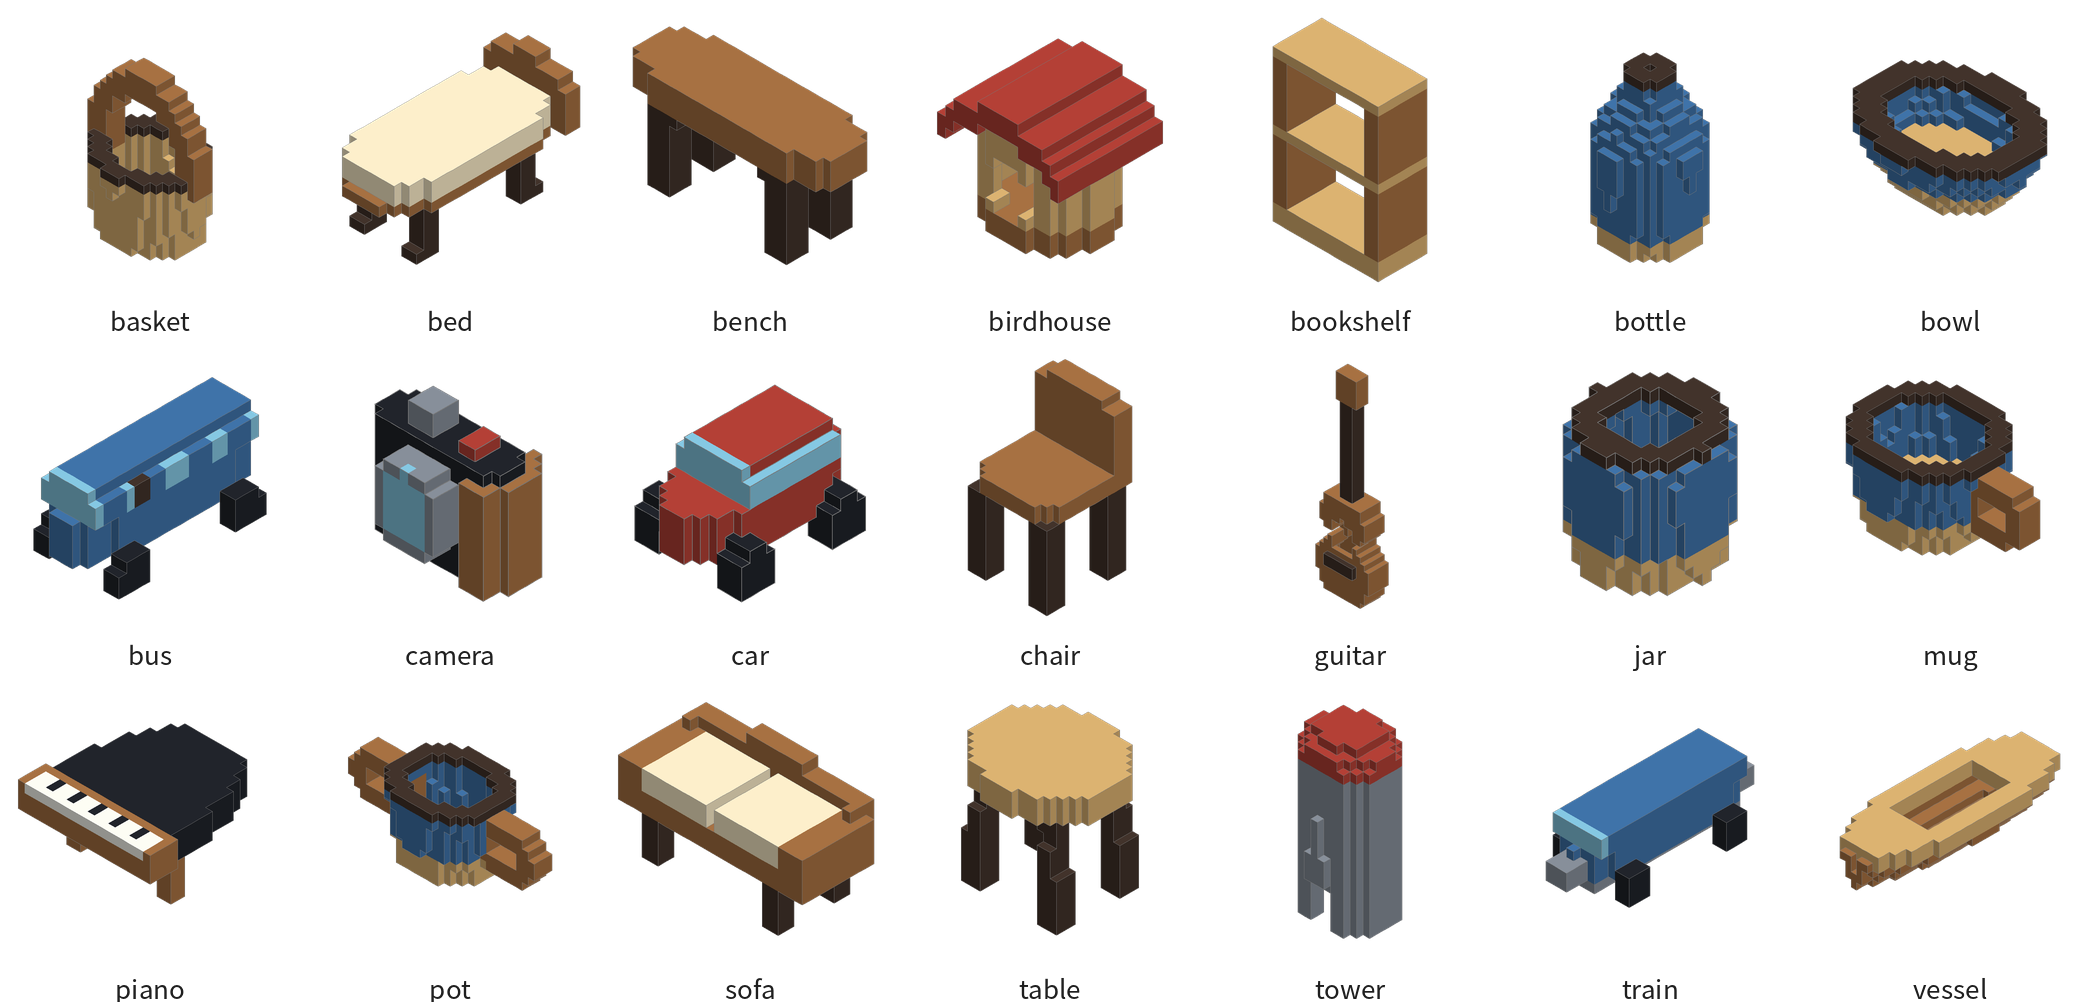
\includegraphics[width=0.475\textwidth]{figures/image7.png}\hfill
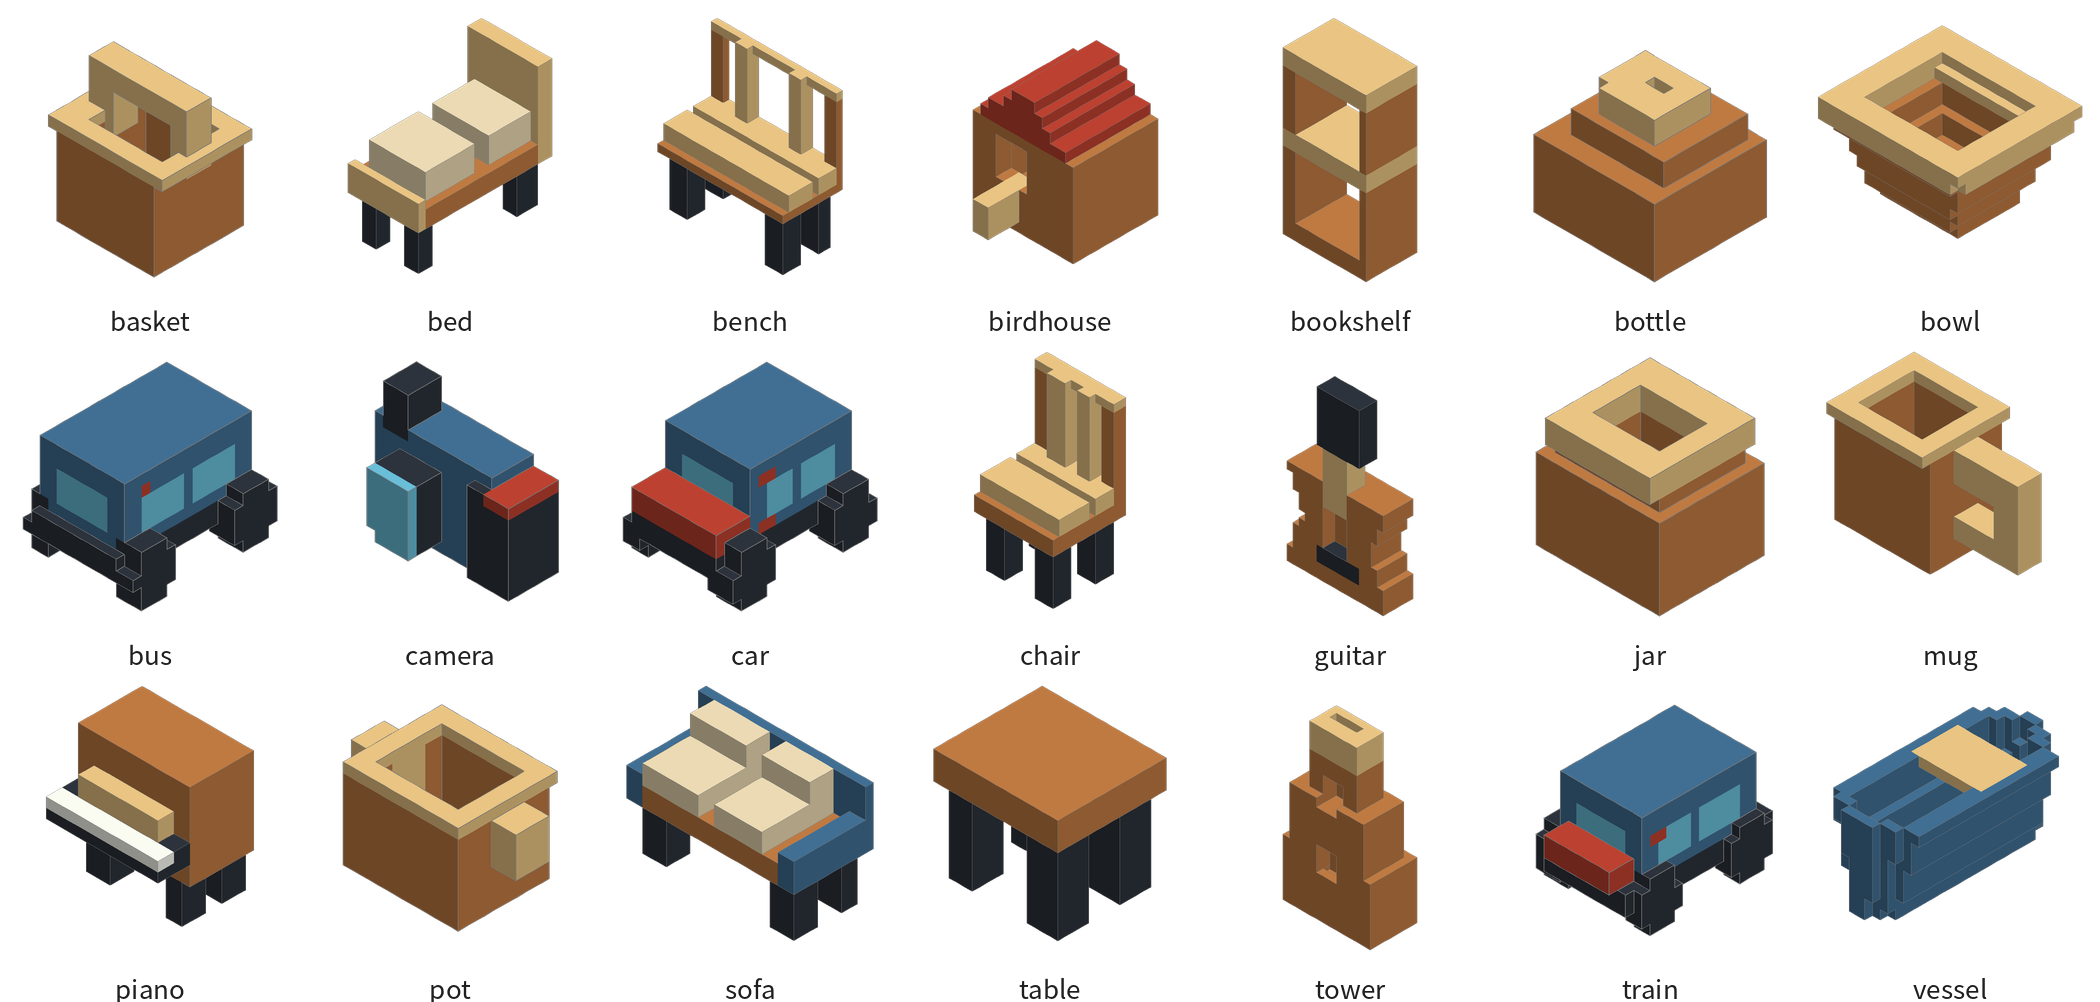
\includegraphics[width=0.475\textwidth]{figures/image8.png}
\caption{Voxel model samples spanning the 21 object categories.}
\end{figure*}

\begin{figure*}[!htbp]
\centering
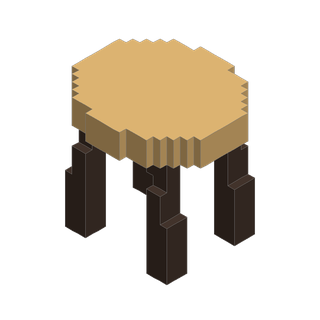
\includegraphics[width=0.118\textwidth]{figures/image4.png}\hfill
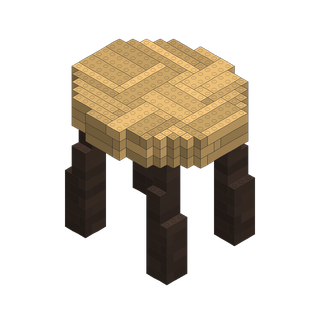
\includegraphics[width=0.118\textwidth]{figures/image5.png}\hfill
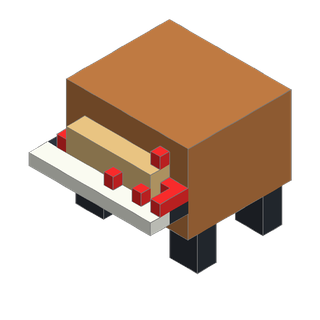
\includegraphics[width=0.118\textwidth]{figures/image2.png}\hfill
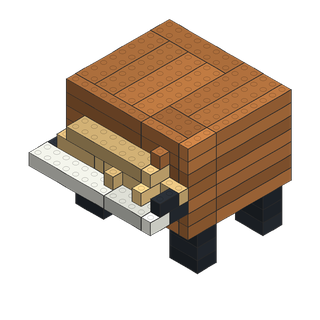
\includegraphics[width=0.118\textwidth]{figures/image3.png}\hfill
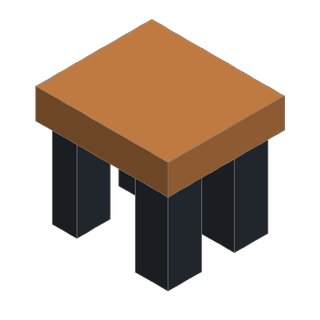
\includegraphics[width=0.118\textwidth]{figures/image9.png}\hfill
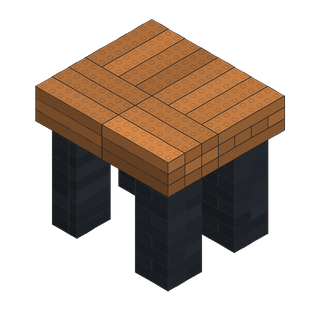
\includegraphics[width=0.118\textwidth]{figures/image10.png}\hfill

\includegraphics[width=0.118\textwidth]{figures/image11.png}\hfill
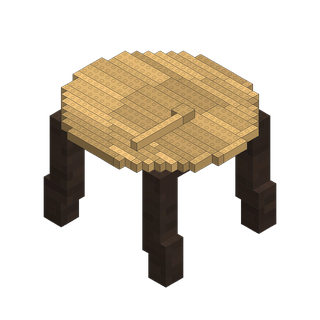
\includegraphics[width=0.118\textwidth]{figures/image12.png}
\caption{Historical examples of voxel targets and brick layouts after local repair.}
\end{figure*}

\begin{figure}[!htbp]
\centering
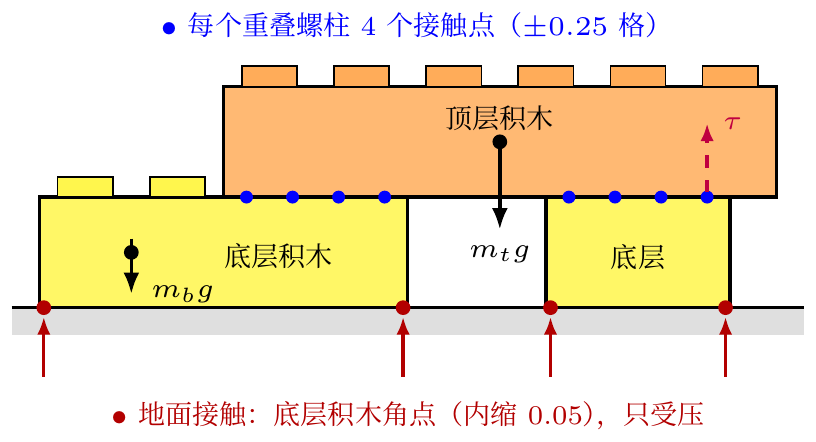
\includegraphics[width=\columnwidth]{figures/image13.png}
\caption{Historical contact-based gravity screening model (source labels in Chinese are retained).}
\end{figure}

\begin{figure*}[!htbp]
\centering
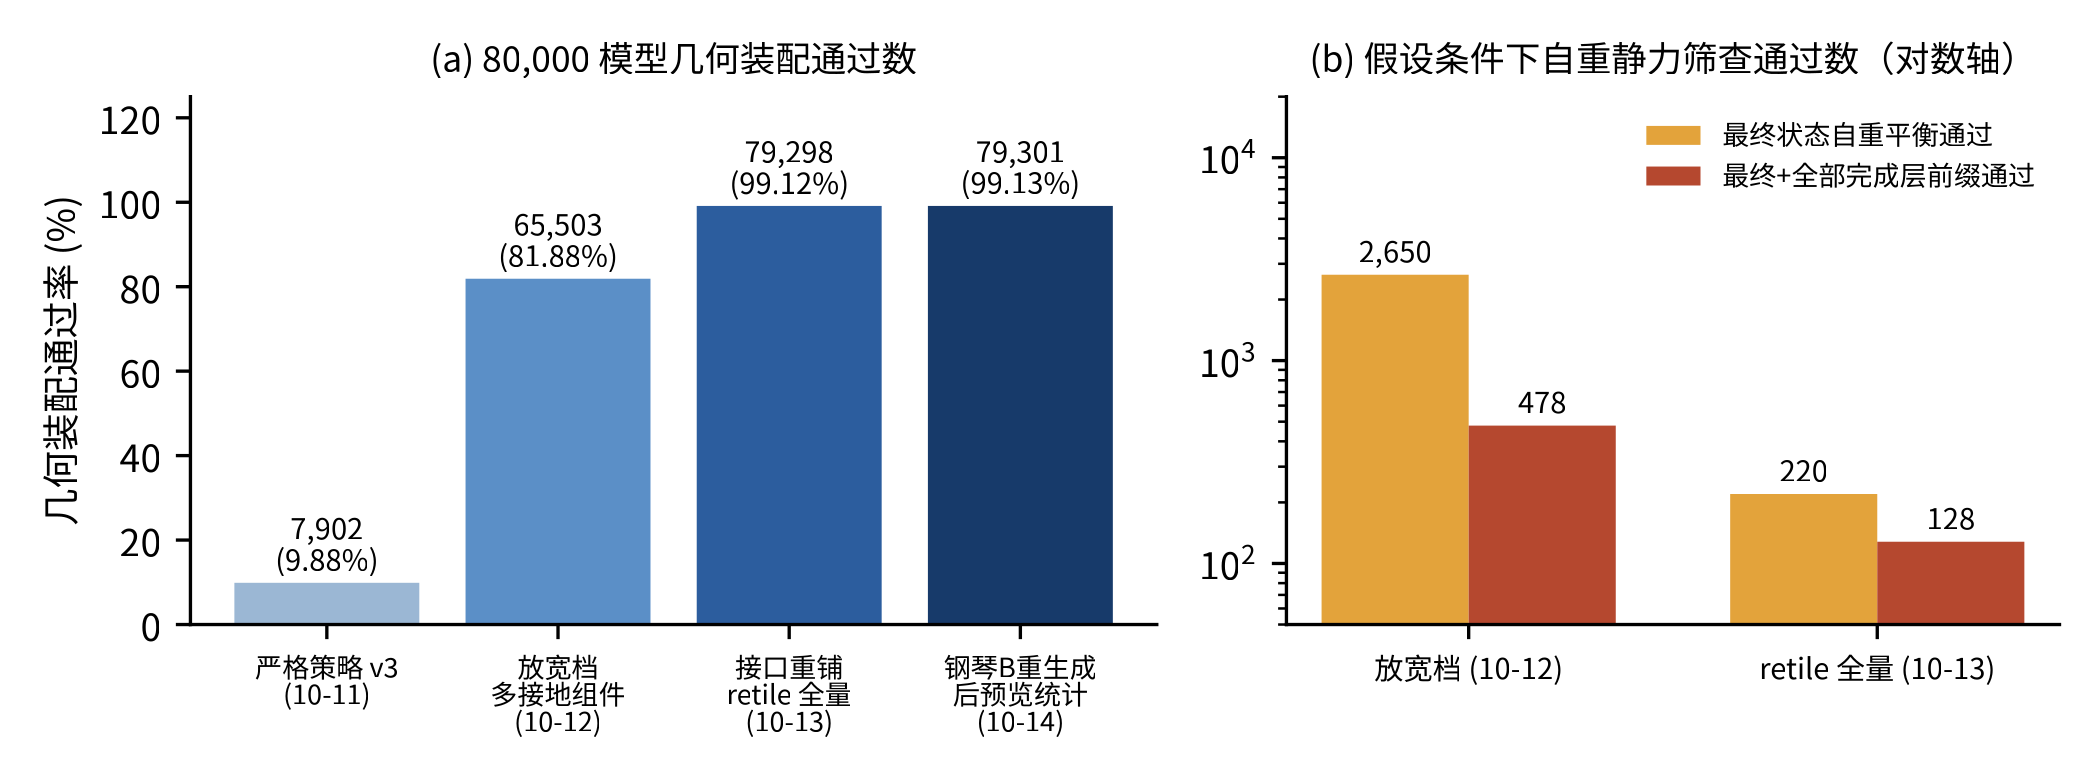
\includegraphics[width=0.85\textwidth]{figures/image14.png}
\caption{Geometric conversion counts and historical screening outcomes. The fourth geometry bar is the report-derived integrated count after piano replacement (Section~\ref{sec:dataset}); the other releases appear in Table~\ref{tab:conversion}. Screening counts refer to the two historical releases shown.}
\end{figure*}

\begin{figure*}[!htbp]
\centering
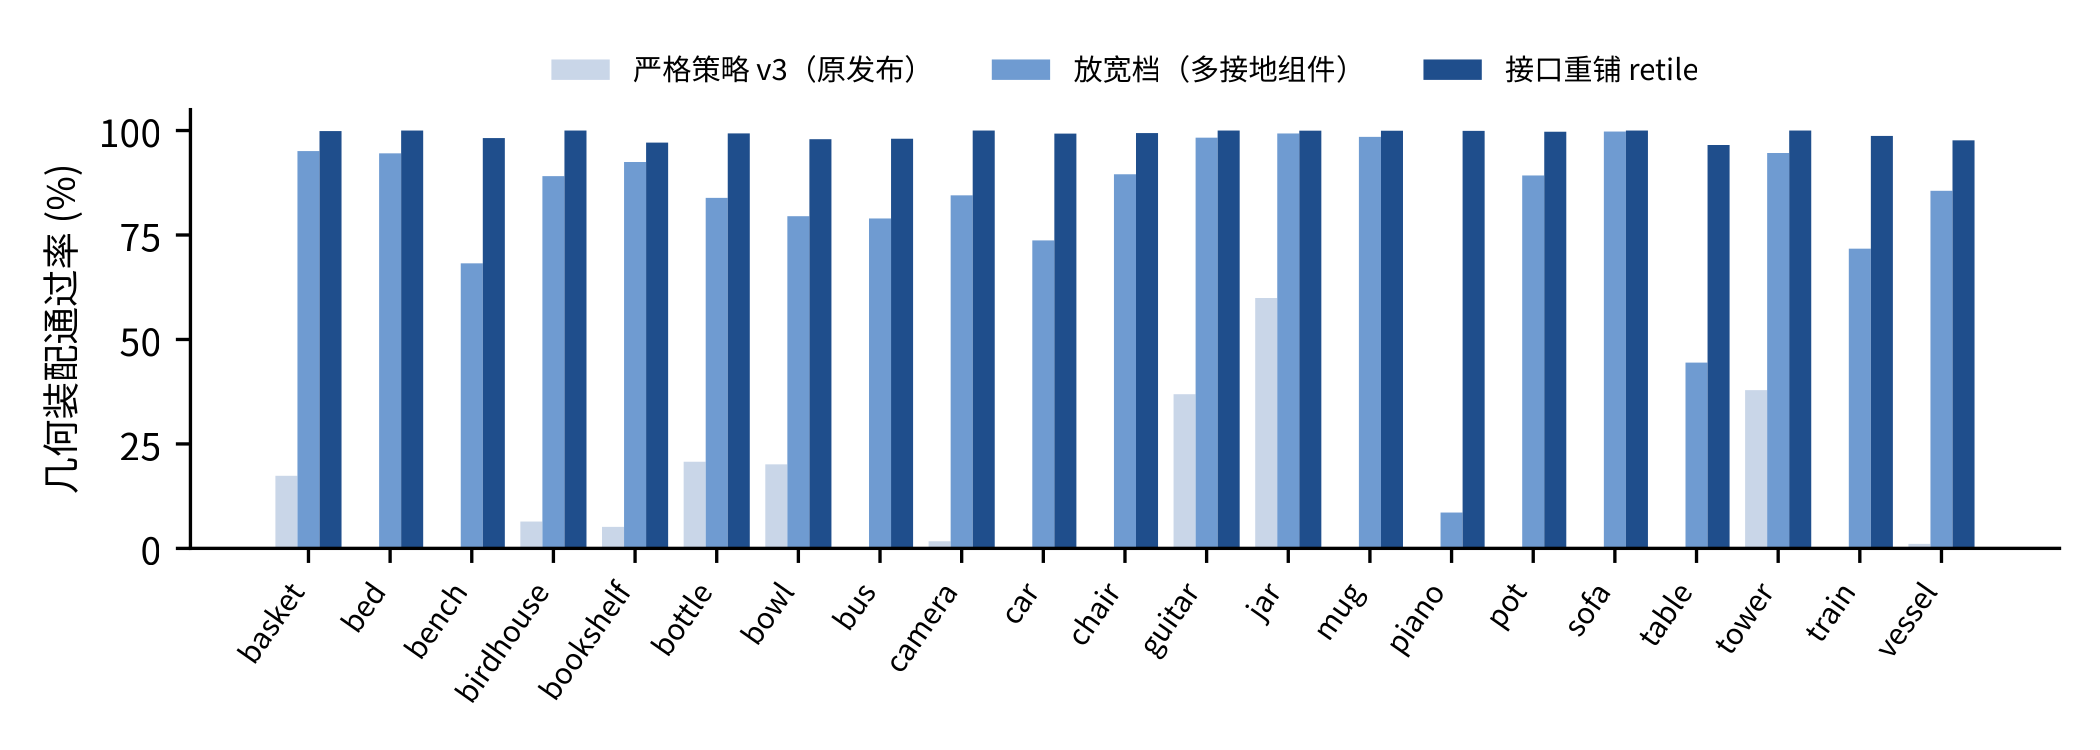
\includegraphics[width=0.85\textwidth]{figures/image15.png}
\caption{Historical category-level geometric pass rates for strict v3, relaxed, and retile releases. Per-category values require verification against version-matched reports.}
\end{figure*}

\begin{figure}[!htbp]
\centering
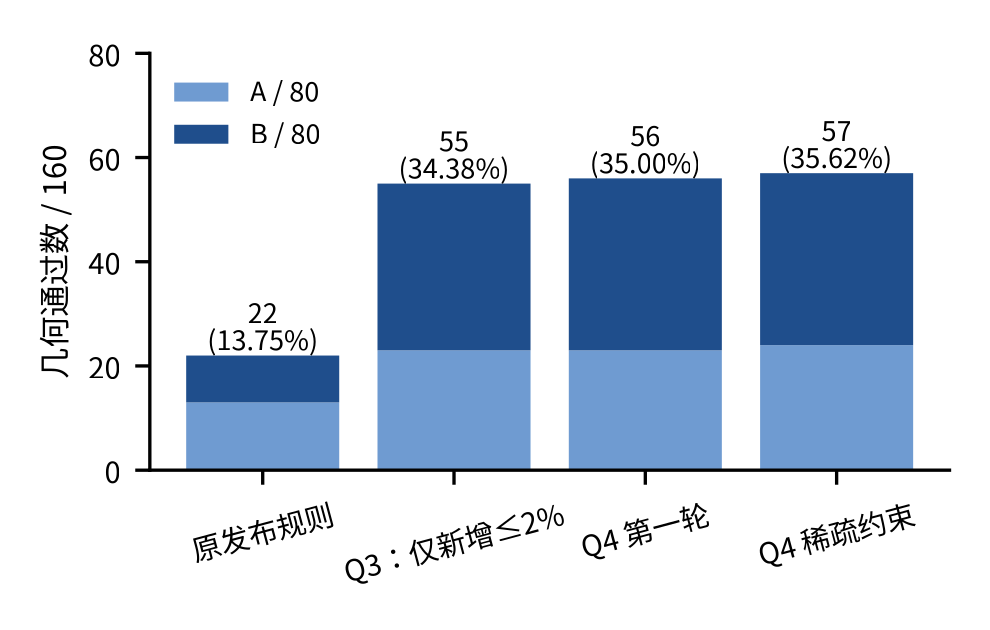
\includegraphics[width=\columnwidth]{figures/image16.png}
\caption{Historical single-stud-component results on a uniform 160-model sample (seed 38177). The Q-series criteria differ from the full-release checks. Per-shard counts and the intermediate Q4 round require verification.}
\end{figure}

\begin{figure*}[!htbp]
\centering
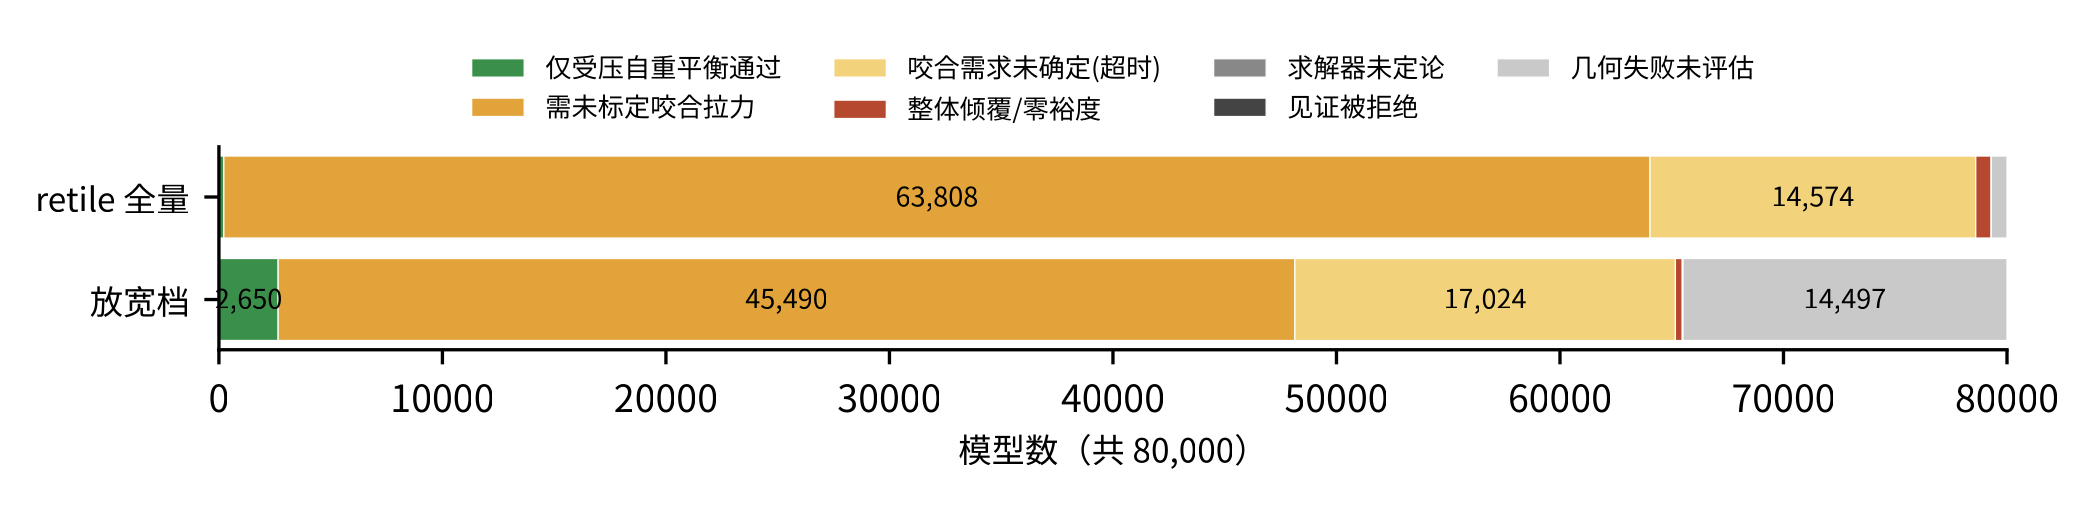
\includegraphics[width=0.85\textwidth]{figures/image17.png}
\caption{Historical distributions of physical screening statuses; values as in the corresponding release reports. Counts refer to the specific releases shown and are kept separate from geometric pass rates.}
\end{figure*}

\FloatBarrier
\section{Technical Appendix: Training Details}
\label{app:training}
Aggregate throughput is 24,448 tokens/s over eight GPUs, and the mean training loss is 0.0273. Evaluation and checkpointing run every 500 steps. With TRL~0.15, the unpacked multi-GPU path hangs after the first backward pass, which is why the TRL~0.17 stack is pinned. Because validation loss is lowest during epoch 2, two epochs would be a more economical setting for future runs (about one third less compute). The full software stack is transformers 4.51.3, trl 0.17.0, peft 0.15.2, datasets 3.6.0, and accelerate 1.6.0, with bf16 precision, gradient checkpointing, and unpacked sequences.

\begin{table}[!htbp]
\centering
\small
\begin{tabular}{lrr}
\toprule
Progress & Step & Validation loss \\
\midrule
Start & 500 & 0.1410 \\
--- & 1,500 & 0.0950 \\
--- & 10,500 & 0.0509 \\
--- & 22,500 & 0.0404 \\
$\approx$ End of epoch 1 & 44,500 & 0.0337 \\
--- & 65,500 & 0.0316 \\
Best (epoch 1.77) & 79,000 & 0.0308 \\
End of epoch 3 & 133,860 & 0.0339 \\
\bottomrule
\end{tabular}
\caption{Validation loss on the 2,000-sample validation subset. One epoch is $\approx$44,620 steps; the nearest evaluation to the end of epoch 1 is step 44,500.}
\label{tab:eval-loss}
\end{table}

% BrickGPT-paper column verified against arXiv:2505.05469 (Sec. 5.1 and Appendix A training details).
\begin{table*}[!htbp]
\centering
\small
\setlength{\tabcolsep}{5pt}
\begin{tabular}{lcc}
\toprule
Dimension & BrickGPT paper & Official Qwen3 script (ours) \\
\midrule
Base model & LLaMA-3.2-1B-Instruct & Qwen3-1.7B \\
LoRA & $r=32$, $\alpha=16$, dropout $0.05$, $q$/$v$ only (3.4M params) & $r=16$, $\alpha=32$, all linear layers \\
Learning rate & $2{\times}10^{-3}$ (AdamW) & $10^{-4}$ \\
Effective batch & 64 & 8 \\
Max length & 4,096 & 8,192 \\
Epochs & 3 & 3 \\
Hardware & 8$\times$RTX A6000, 12\,h & 8$\times$4090D, 25.3\,h \\
Data & StableText2Brick, 47k structures / 240k prompts & BrickMore-48, 79.3k models / 396,610 samples \\
\bottomrule
\end{tabular}
\caption{Our configuration versus the original BrickGPT paper \cite{brickgpt}. BrickGPT-paper values are taken from Sec.~5.1 and Appendix~A of arXiv:2505.05469 (base model, LoRA $r{=}32$, $\alpha{=}16$, dropout $0.05$, $q$/$v$ only with 3.4M parameters, AdamW learning rate $0.002$, global batch 64, 4096-token length filter, 3 epochs, 8$\times$RTX A6000 and 12\,h, and 47k+ structures / 240k prompts). The data organization, instruction template, absence of thinking mode, and LoRA paradigm follow BrickGPT; concrete hyperparameters follow the official Qwen3 adaptation, with the budget adjusted for the larger world, library, and corpus.}
\label{tab:brickgpt-recipe}
\end{table*}

\FloatBarrier
\section{Technical Appendix: Additional Evaluation Material}
\label{app:eval}

\emph{Baseline run configuration.} BrickGPT outputs were generated in a $20^3$ world with seed 42. Run records report \texttt{max\_regen}=8 and \texttt{use\_gurobi}=\texttt{False} for all 114 prompts, which differ from the BrickGPT paper (up to 100 physics-aware rollbacks; the stability program in Eqn.~3 is solved with Gurobi) and from the official repository defaults (\texttt{max\_regenerations}=100, \texttt{use\_gurobi}=\texttt{True}), assuming \texttt{max\_regen} denotes the rollback limit \texttt{max\_regenerations}. With Gurobi disabled, the recorded stability flag reflects the repository's connectivity-based check rather than its physical-stability analysis. We therefore do not describe this run as using the authors' default configuration.

\emph{Paired tests.} Table~\ref{tab:sig} re-analyzes the existing per-prompt scores of the main comparison. Pairs are formed by prompt (114 prompts, one output per system); differences are BrickForma minus the opponent. The sign test is a two-sided exact binomial test on wins versus losses (no ties occurred); the Wilcoxon signed-rank test is two-sided with the normal approximation. Holm correction is applied over the six comparisons (three metrics $\times$ two opponents), separately for each test; $P_{\mathrm{inv}}$ is not tested. Because the delivered outputs differ in candidate selection (Section~\ref{sec:setup}), the tests describe these outputs, not isolated model capability.

\begin{table}[!htbp]
\centering
\small
\setlength{\tabcolsep}{3pt}
\begin{tabular}{llrrrr}
\toprule
vs. & Metric & W/L & Sign $p_{\mathrm{H}}$ & $W$ & Wilc.\ $p_{\mathrm{H}}$ \\
\midrule
BrickGPT & VQAScore & 91/23 & $1.9{\times}10^{-10}$ & 898 & $3.4{\times}10^{-11}$ \\
BrickGPT & PE & 95/19 & $7.3{\times}10^{-13}$ & 433 & $4.4{\times}10^{-15}$ \\
BrickGPT & SigLIP2 & 91/23 & $1.9{\times}10^{-10}$ & 1129 & $1.2{\times}10^{-9}$ \\
BrickNet & VQAScore & 97/17 & $3.5{\times}10^{-14}$ & 843 & $1.8{\times}10^{-11}$ \\
BrickNet & PE & 98/16 & $7.4{\times}10^{-15}$ & 275 & $1.3{\times}10^{-16}$ \\
BrickNet & SigLIP2 & 102/12 & $3.6{\times}10^{-18}$ & 740 & $2.9{\times}10^{-12}$ \\
\bottomrule
\end{tabular}
\caption{Paired two-sided tests of BrickForma against each baseline on 114 prompts (W/L: prompts on which BrickForma scores higher/lower; $W$: Wilcoxon statistic; $p_{\mathrm{H}}$: Holm-adjusted two-sided $p$). All Holm-adjusted $p$ values are below $1.3{\times}10^{-9}$.}
\label{tab:sig}
\end{table}

\begin{table}[!htbp]
\centering
\small
\setlength{\tabcolsep}{3pt}
\begin{tabular}{llrrr}
\toprule
Level ($n$) & System & VQAScore & PE & SigLIP2 \\
\midrule
L1 (21) & BrickForma & \textbf{0.2201} & \textbf{0.1693} & \textbf{0.0478} \\
 & BrickGPT & 0.1085 & 0.1364 & 0.0173 \\
 & BrickNet & 0.0833 & 0.1151 & 0.0035 \\
\midrule
L2 (21) & BrickForma & \textbf{0.3615} & \textbf{0.1763} & \textbf{0.1027} \\
 & BrickGPT & 0.2507 & 0.1415 & 0.0331 \\
 & BrickNet & 0.0283 & 0.1178 & 0.0135 \\
\midrule
L3 (23) & BrickForma & \textbf{0.2364} & \textbf{0.1839} & \textbf{0.1386} \\
 & BrickGPT & 0.1711 & 0.1433 & 0.0376 \\
 & BrickNet & 0.0714 & 0.1301 & 0.0126 \\
\midrule
L4 (25) & BrickForma & \textbf{0.1935} & \textbf{0.2000} & \textbf{0.1682} \\
 & BrickGPT & 0.1078 & 0.1535 & 0.0302 \\
 & BrickNet & 0.0902 & 0.1475 & 0.0176 \\
\midrule
L5 (24) & BrickForma & \textbf{0.0968} & \textbf{0.1947} & \textbf{0.1447} \\
 & BrickGPT & 0.0748 & 0.1519 & 0.0293 \\
 & BrickNet & 0.0363 & 0.1363 & 0.0023 \\
\bottomrule
\end{tabular}
\caption{Main-comparison means by description level (same 114 prompts as Table~\ref{tab:main}).}
\label{tab:levels}
\end{table}

\begin{table}[!htbp]
\centering
\small
\setlength{\tabcolsep}{3pt}
\begin{tabular}{lr}
\toprule
Quantity (525 prompts) & Value \\
\midrule
Raw layout is a single stud component & 46 (8.8\%) \\
Stud components per failing raw (med./max) & 5 / 33 \\
Failing raw layouts with duplicated voxels & 50 / 479 \\
Detached fragments (airborne / grounded) & 1,320 / 920 \\
MILP tier reached (12 / 60 / 180 / 600\,s) & 326 / 133 / 18 / 2 \\
Prompts resampled outside $S$ & 28 \\
Final: single stud comp., union unchanged & 525 / 525 \\
Raw bricks, median (range) & 183 (77--623) \\
Final assembly bricks, median & 452 \\
\bottomrule
\end{tabular}
\caption{Structural diagnostics of raw outputs (Section~\ref{sec:diagnostics}). ``Union unchanged'' means the final assembly covers exactly the in-bounds voxel union of the raw draft; it does not assess whether the shape matches the prompt.}
\label{tab:diag}
\end{table}

% image18 removed from the submitted PDF per user decision (V1.6, U4-b); figures/image18.png is kept.
\iffalse
\begin{figure*}[!htbp]
\centering
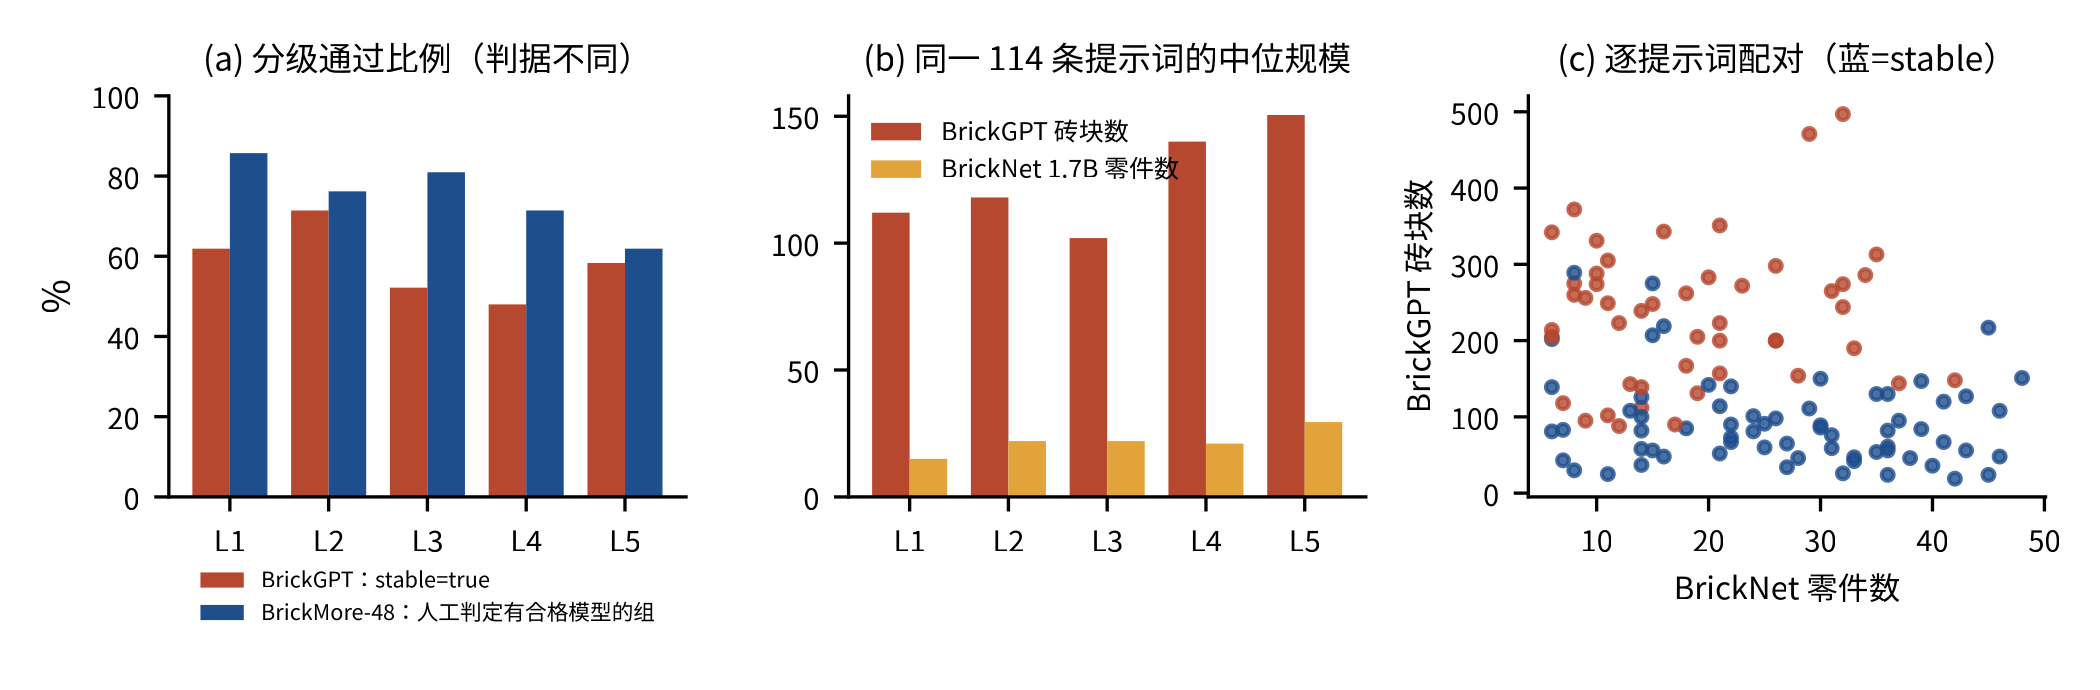
\includegraphics[width=0.85\textwidth]{figures/image18.png}
\caption{Historical baseline comparison with differing acceptance criteria; not the current matched main comparison.}
\end{figure*}
\fi

\begin{figure*}[!htbp]
\centering
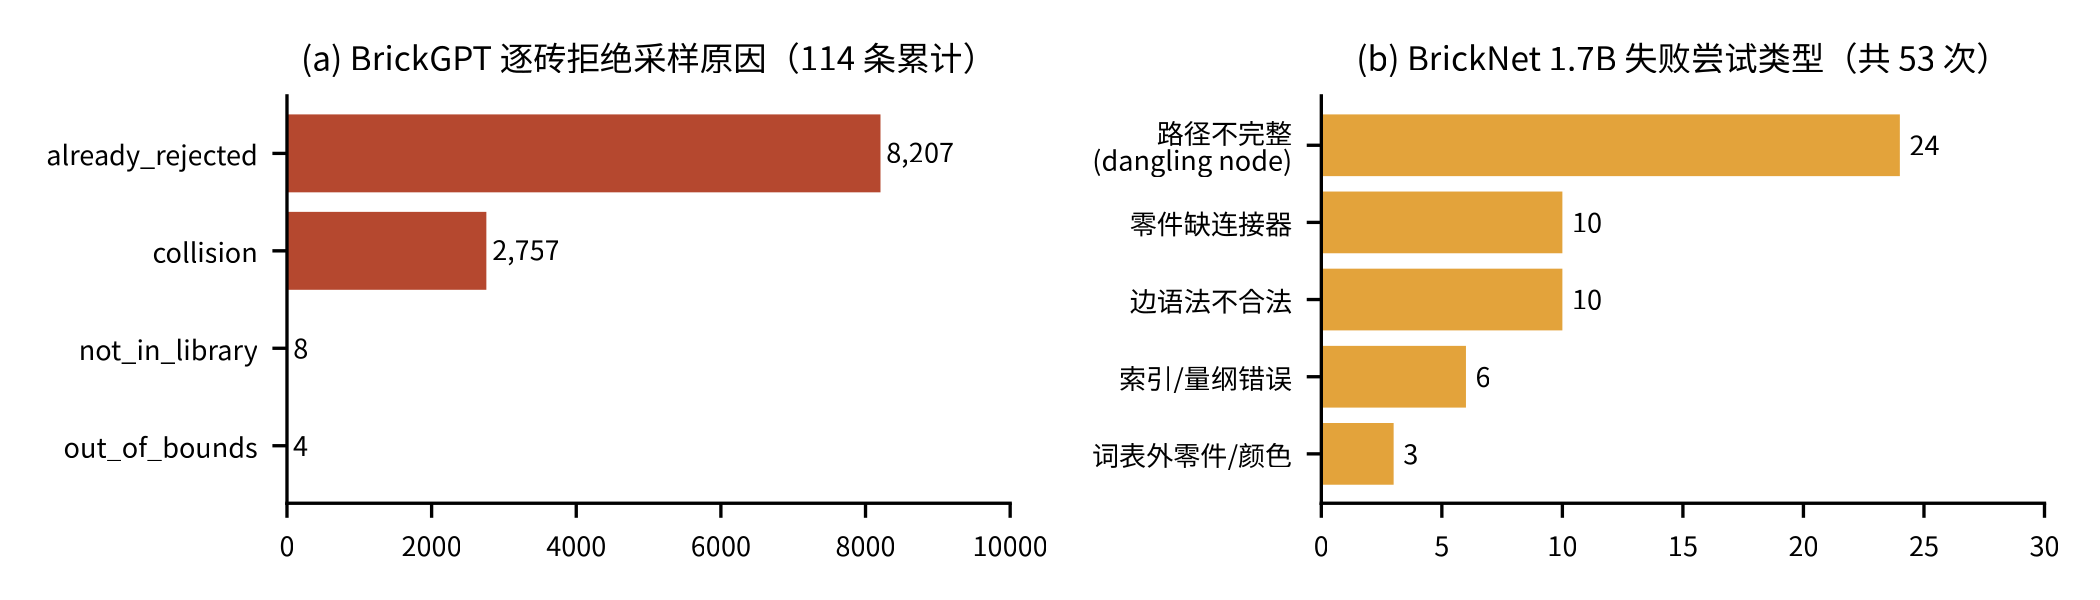
\includegraphics[width=0.85\textwidth]{figures/image19.png}
\caption{Historical rejection-event counts across 114 BrickGPT runs (left) and categories of 53 failed BrickNet attempts (right), as shown in the supplied reference.}
\end{figure*}

\begin{figure*}[!htbp]
\centering
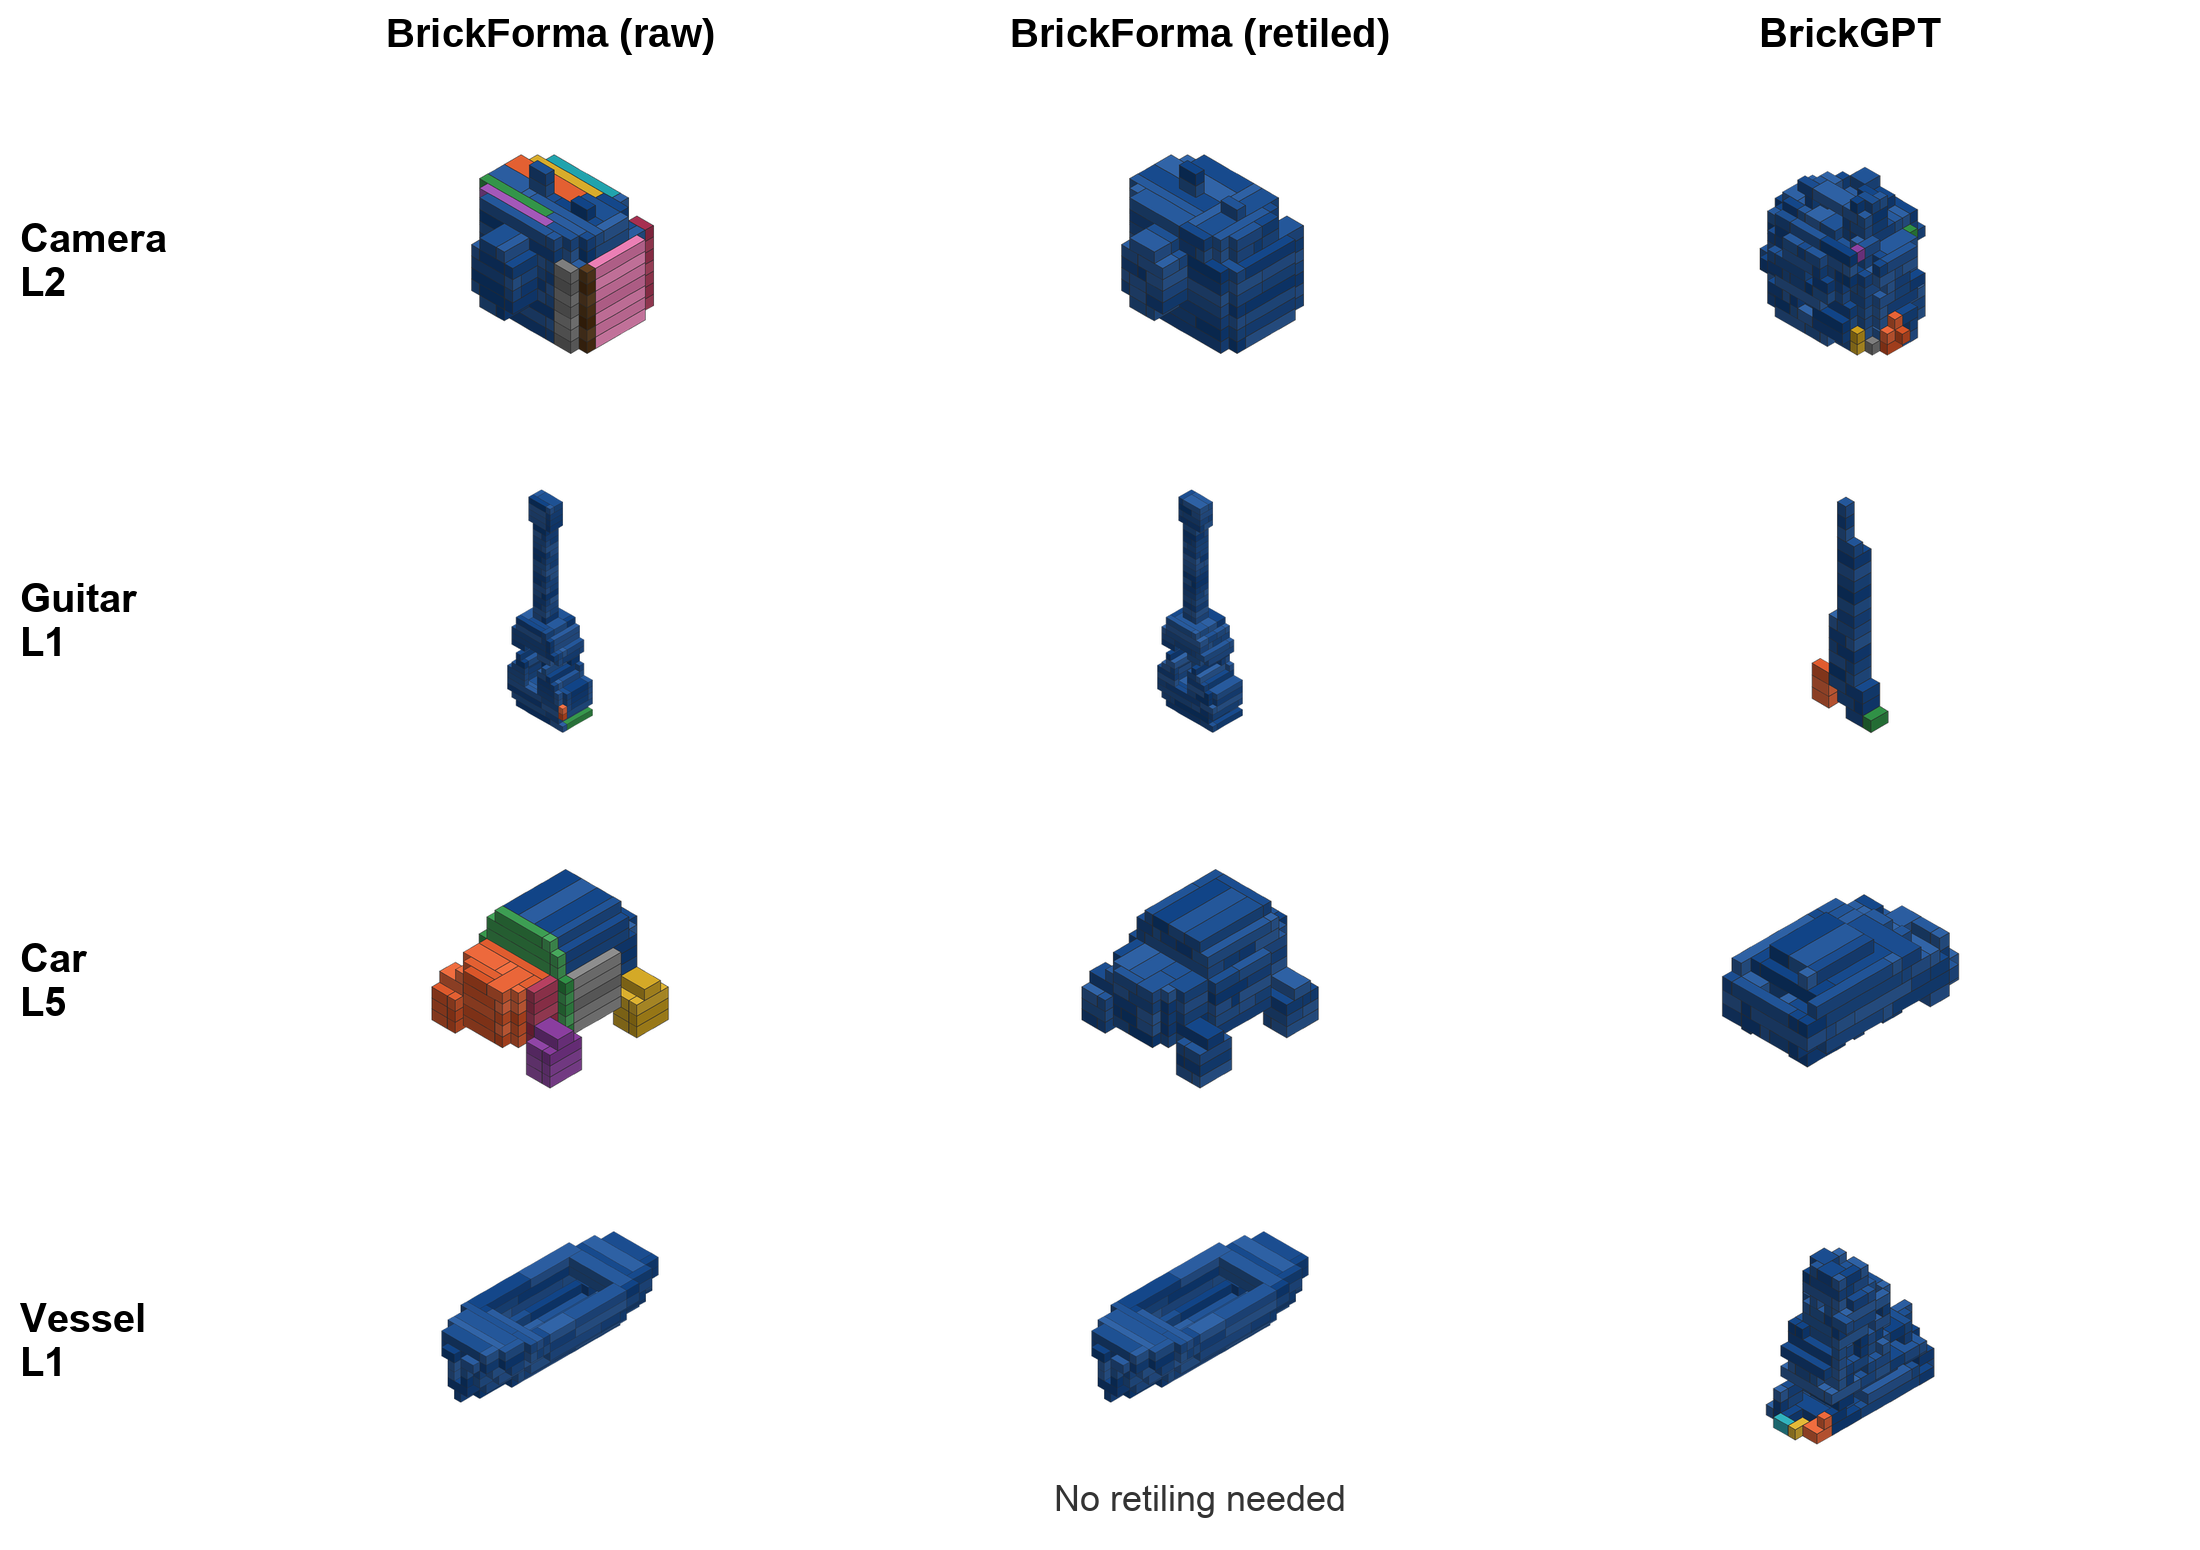
\includegraphics[width=0.85\textwidth]{figures/original_comparison.png}
\caption{Qualitative historical examples from the supplied reference. Columns show raw and retiled outputs of our system and BrickGPT outputs.}
\end{figure*}

\FloatBarrier
\section{Technical Appendix: Historical Tables}
\label{app:historical}
The following transcribed tables preserve the historical reference material. They use different versions or evaluation criteria and are not substitutes for the current main comparison. Where a value is superseded by a verified number in the main text (e.g., Table~\ref{tab:training-data} and Appendix~\ref{app:dataset}), the main text takes precedence. Dashes indicate missing entries in the supplied source.
\begin{table*}[!htbp]\centering\small
\begin{tabular}{lr}\toprule
Item & Historical value \\ \midrule
Voxel models & 80,000 (40,000 per batch) \\
Categories / structural families & 21 / 40 per category \\
Grid / voxel count & $48^3$ / 750--1,250 \\
Prompt records & 400,000 (five bilingual records per model) \\
Uniqueness & 80,000 unique; 0 A/B duplicates \\
Overlap with historical hashes & 0 / 55,255 \\
Retile geometry passes & 79,298 (99.12\%) \\
Bricks in full preview & 12,718,389 \\
Final gravity equilibrium passes & 220 \\
Final and layer-prefix passes & 128 \\
\bottomrule\end{tabular}
\caption{Historical dataset statistics transcribed from the supplied reference. The geometry count refers to the old retile release, not the later integrated count. Verify the preview and physical-screening totals against version-matched reports.}
\end{table*}

\begin{table*}[!htbp]\centering\scriptsize
\begin{tabular}{llrrrrr}\toprule
Version & Connectivity & Voxel changes & Passes & Rate & Final & Final + prefixes \\ \midrule
Strict v3 & Single; support $\geq$10\%, overhang $\leq$2 & None & 7,902 & 9.88\% & -- & -- \\
Relaxed & Each component grounded & +428,278 / -38,230 & 65,503 & 81.88\% & 2,650 & 478 \\
Retile & Each component grounded & +228,582 / -125 & 79,298 & 99.12\% & 220 & 128 \\
\midrule
\multicolumn{7}{l}{Uniform 160-model sample (seed 38177); not full-dataset results} \\
Baseline & Single stud-connected component & None & 22 & 13.75\% & -- & -- \\
Q3 & Single stud-connected component & Added $\leq$2\% & 55 & 34.38\% & 8 & 2 \\
Q4 (sparse) & Single stud-connected component & Added + removed $\leq$2\% & 57 & 35.63\% & 8 & 2 \\
\bottomrule\end{tabular}
\caption{Historical conversion-strategy table from the reference. Full-dataset and 160-model sample rows use different scopes; connectivity rules also differ. Final and prefix columns report screening outcomes under the stated historical assumptions.}
\end{table*}

\begin{table*}[!htbp]\centering\small
\begin{tabular}{lrrr}\toprule
Item & BrickGPT & BrickNet 1.7B & BrickMore-48 \\ \midrule
Representation & $20^3$ bricks & Assembly graph & $48^3$ bricks \\
Criterion & stable & Parseable & -- \\
Passes & 66/114 & 114/114 & -- \\
Median parts & 126.5 & 22 & -- \\
Range & 19--497 & 6--48 & -- \\
Mean time (s) & 189.6 & -- & -- \\
\bottomrule\end{tabular}
\caption{Historical baseline table in the source reference. These criteria differ, and missing BrickMore-48 entries were marked TODO. This is not the current matched four-metric main table.}
\end{table*}

\begin{table*}[!htbp]\centering\small
\begin{tabular}{lrrrrl}\toprule
Level & $n$ & BrickGPT stable & BrickGPT median bricks & BrickNet median parts & BrickMore-48 \\ \midrule
L1 & 21 & 13 & 112 & 15 & -- \\
L2 & 21 & 15 & 118 & 22 & -- \\
L3 & 23 & 12 & 102 & 22 & -- \\
L4 & 25 & 12 & 140 & 21 & -- \\
L5 & 24 & 14 & 150.5 & 29.5 & -- \\
\bottomrule\end{tabular}
\caption{Historical level-wise baseline table transcribed from the reference. The original BrickMore-48 column was incomplete, and the other columns use different criteria.}
\end{table*}

\begin{table*}[!htbp]\centering\small
\begin{tabular}{lrrrr}\toprule
Method and source & $P_{\mathrm{inv}}$ & VQA & PE & SigLIP2 \\ \midrule
BrickGPT (literature, as transcribed) & 0.063 & 0.050 & 0.157 & 0.052 \\
BrickNet 1.7B (literature, as transcribed) & 0.260 & 0.593 & 0.282 & 0.631 \\
BrickGPT (114 prompts, historical placeholder) & -- & -- & -- & -- \\
BrickNet (114 prompts, historical placeholder) & -- & -- & -- & -- \\
BrickMore-48 (114 prompts, historical placeholder) & -- & -- & -- & -- \\
\bottomrule\end{tabular}
\caption{Original reference table with literature values and historical placeholders. Literature values use another evaluation set and must not be directly compared with the present 114-prompt results; the precise $P_{\mathrm{inv}}$ definition and direction require checking against the original publication.}
\end{table*}


\FloatBarrier
\end{document}
